%%%%%%%%%%%%%%%%%%%%%%%%%%%%%%%%%%%%%%%%%%%%%%%%%%%%%%%%%%%%%%%%%%%%%%%%%%%%%%%%%%%%%%%%%%%%%%%%%%%%%%%
% PACKAGES

\documentclass[a4paper, 11pt]{article}
\usepackage[utf8]{inputenc}
\usepackage[T1]{fontenc}
%\usepackage[catalan]{babel}
\usepackage{amsmath, amssymb, amsthm}
\usepackage[margin=1in]{geometry}
\usepackage{enumerate}
\usepackage{array}
\usepackage{graphicx}
\usepackage{ragged2e}
\usepackage{subfig}
\usepackage{caption}
\usepackage{subcaption}
\usepackage[dvipsnames]{xcolor}
\usepackage{float}
\usepackage{chngcntr}
\usepackage{ragged2e}
\usepackage{multirow}
\usepackage{vmargin}
\usepackage{hyperref}
\usepackage{url}
\usepackage{fancyhdr}
\usepackage{bigints}
\usepackage{listings}
\usepackage{xcolor,colortbl}
\usepackage{mathrsfs}

%%%%%%%%%%%%%%%%%%%%%%%%%%%%%%%%%%%%%%%%%%%%%%%%%%%%%%%%%%%%%%%%%%%%%%%%%%%%%%%%%%%%%%%%%%%%%%%%%%%%%%%
% COLORS

\definecolor{bluebell}{rgb}{0.64, 0.64, 0.82}
\definecolor{atomictangerine}{rgb}{1.0, 0.6, 0.4}
\definecolor{applegreen}{rgb}{0.55, 0.71, 0.0}
\definecolor{frenchblue}{rgb}{0.0, 0.45, 0.73}
\definecolor{darkpastelgreen}{rgb}{0.01, 0.75, 0.24}
\definecolor{darkpastelblue}{rgb}{0.47, 0.62, 0.8}
\definecolor{navy}{rgb}{0,0,128}
\definecolor{codegreen}{rgb}{0,0.6,0}
\definecolor{codegray}{rgb}{0.5,0.5,0.5}
\definecolor{codepurple}{rgb}{0.58,0,0.82}
\definecolor{backcolour}{rgb}{0.95,0.95,0.92}
\definecolor{amaranth}{rgb}{0.9, 0.17, 0.31}
\definecolor{GRAY}{rgb}{0.75, 0.75, 0.75}
\definecolor{deepfuchsia}{rgb}{0.76, 0.33, 0.76}
\definecolor{deepmagenta}{rgb}{0.8, 0.0, 0.8}
\definecolor{funcblue}{rgb}{0.36, 0.57, 0.9}

%%%%%%%%%%%%%%%%%%%%%%%%%%%%%%%%%%%%%%%%%%%%%%%%%%%%%%%%%%%%%%%%%%%%%%%%%%%%%%%%%%%%%%%%%%%%%%%%%%%%%%%
% SETTINGS

% COLOR LINK/REFERENCES
\hypersetup{colorlinks=true,
            linkcolor=blue,
            filecolor=magenta,      
            urlcolor=blue,
            }

% PAGE'S STYLE OF INITIAL PAGES
\fancypagestyle{plain}{
    \lhead[]{} % left part of the header
    \rhead[]{} % right part of the header
    \fancyfoot[]{} % borrow the foot counter page
    \lfoot[]{} % left part of the footpage
    \rfoot[]{} % right part of the footpage
    \renewcommand{\headrulewidth}{0pt} % separator line of the header
    \renewcommand{\footrulewidth}{0.5pt} % separator line of the footpage
}

% PAGE'S STYLE FOR THE THESIS
\fancypagestyle{extended_plain}{
    \lhead[]{Gerard Lahuerta Martín} % left part of the header
    \rhead[]{\leftmark} % right part of the header
    \fancyfoot[]{} % borrow the foot counter page
    \lfoot[]{} % left part of the footpage
    \rfoot[]{\thepage} % right part of the footpage
    \renewcommand{\headrulewidth}{0.5pt} % separator line of the header
    \renewcommand{\footrulewidth}{0.5pt} % separator line of the footpage
}

%%%%%%%%%%%%%%%%%%%%%%%%%%%%%%%%%%%%%%%%%%%%%%%%%%%%%%%%%%%%%%%%%%%%%%%%%%%%%%%%%%%%%%%%%%%%%%%%%%%%%%%
% CODE STYLE


%%%%%%%%%%%%%%%%%%%%%%%%%%%%%%%%%%%%%%%%%%%%%%%%%%%%%%%%%%%%%%%%%%%%%%%%%%%%%%%%%%%%%%%%%%%%%%%%%%%%%%%
% DOCUMENT

\begin{document}
\pagestyle{plain}

% TITLE
\begin{titlepage}
    \centering
    {
\includegraphics[width=0.4\textwidth]{PORTADA/UAB.png}\par}
    \vspace{1cm}
    {\bfseries\LARGE \href{https://www.uab.cat/}{Universitat Autònoma de Barcelona} \par}
    \vspace{2cm}
    {\Large Degree Thesis \par}
    \vspace{2em}
    \rule{\linewidth}{0.4pt}\\
    \vspace{1cm}
    {\scshape\Huge \textbf{Improvements of Deterministic Processes through Neural Networks} \par}
    \vspace{1cm}
    \rule{\linewidth}{0.4pt}\\
    \vspace{2cm}
    {\Large
    \begin{figure}[h]
    \centering
        \begin{minipage}{5cm} \centering % Minipagina para la tabla. 8 cm de ancho
            \begin{tabular}{c}
                Author: \\
                \href{https://github.com/Gerard-Lahuerta}{Gerard Lahuerta Martín}
            \end{tabular}
        \end{minipage}
        \hspace{3em}
        \begin{minipage}{5cm} \centering % Minipagina para la tabla. 8 cm de ancho
            \begin{tabular}{c}
                Supervisor: \\
                \href{https://mat.uab.cat/~alseda/}{Dr. Lluís Alsedà Soler}
            \end{tabular}
        \end{minipage}
    \end{figure}\par}
    \vspace{2cm}
    {\scshape 
        \begin{minipage}{10cm} \centering % Minipagina para la tabla. 8 cm de ancho
            A thesis submitted in fulfilment of the requirements
            for the degree of Computational Mathematics and Data Analytics in the
        \end{minipage} 
    \par} 
    \vspace{2em}
    {\scshape\Large \href{https://www.uab.cat/ciencies}{science faculty} \par}
    \vfill
    {\Large June 2024 \par}
\end{titlepage}


\justifying
\newpage
\textcolor{white}{a}
\newpage 

% PRE SECTIONS
\section*{Declaration of Authorship}
I, \textit{Gerard Lahuerta Martín}, declare that this thesis titled, "\textbf{Improvements of Deterministic Processes through Neural Networks}" and the work presented in it are my own. I confirm that:
\begin{itemize}
    \item This work was done wholly or mainly while in candidature for a bachellor degree
    at this University.
    \item Where any part of this thesis has previously been submitted for a degree or
    any other qualification at this University or any other institution, this has been
    clearly stated.
    \item Where I have consulted the published work of others, this is always clearly
    attributed.
    \item Where I have quoted from the work of others, the source is always given. With
    the exception of such quotations, this thesis is entirely my own work.
    \item I have acknowledged all main sources of help.
    \item Where the thesis is based on work done by myself jointly with others, I have
    made clear exactly what was done by others and what I have contributed myself.
\end{itemize}
\textcolor{white}{a}\\
\underline{Signed: \hspace{7em} \textsl{\texttt{Gerard.}} \hspace{7em}}\\
\textcolor{white}{a}\\
\underline{Date: \hspace{7em} 21-06-2024 \hspace{7em}}


\newpage
\section*{Abstract}
This study in the context of neural networks and computational cost gives a new perspective of a possible method that reduces time-cost of deterministic processes.\\
Its main objective is to sample enough evidence for which deterministic processes can be modelled with neural networks, allowing in cases where this deterministic processes are computationally expensive come by an approximated value within a fixed time.\\
This study is performed using the scientific method of: \textit{Observation}, \textit{Hypothesis}, \textit{Experimentation}, \textit{Conclusions}.\\
It develops some working hypotheses that could not be proven but if future investigations verify it, these working hypotheses gives a better understanding of neural networks and how their architecture can be planned.\\
The results are not as relevant as should be to ensure the viability of the Working Hypothesis proposet but they give a starting point for future works in the area.\\
\textcolor{white}{a}\\
\textcolor{white}{a}\\
\underline{\textbf{Key words:}} \textit{neural networks, multilayer perceptron, deterministic process, Universal Approximation Theorem, distribution of roman numbers.}

\newpage
\section*{Acknowledgements}
I want to thank my family for their support throughout my thesis, degree, and life.\\
\textcolor{white}{a}\\
I am especially grateful to my mother, Maria Montserrat, for her encouragement and guidance in facing the challenges of this thesis and my career.\\
\textcolor{white}{a}\\
Thanks to everyone who treated me as if I was part of their family.\\
\textcolor{white}{a}\\
I also appreciate the encouragement and support of my colleagues.\\
\textcolor{white}{a}\\
Finally, I want to give a special mention to Dr. Lluís Alsedà for guiding me through the thesis and being an inspiration.\\
\textcolor{white}{a}\\
Thank you all for everything.
\newpage

% CONTENTS
\tableofcontents
\listoffigures
\listoftables

\newpage
\section*{Preface}
This report is an ambitious project that has been developing for months and has been meditated even more.\\
Every result obtained remarks the viability of neural network development and how it can be implemented to solve problems that have high computational costs.\\
All the resources used can be consulted in the \href{https://github.com/Gerard-Lahuerta/TFG}{GitHub repository}.

\newpage \pagestyle{extended_plain}
\setcounter{page}{2}
\addcontentsline{toc}{section}{Introduction}
\section*{Introduction}
This work is a starting point for other investigations about neural networks in deterministic processes and how they can be developed.\\
It is known that a fixed series of rules which associates two groups can be explained as an application between these sets.
This application is unknown and in some cases cannot be described at all. Nevertheless, since the deterministic process exists, it is possible to create some registers to train a neural network.\\
This neural network, thanks to the \textbf{Universal Approximation Theorem}, can mimic the application, with enough time and data. Therefore, it can approach the results of the deterministic process.\\
In cases where it is not possible to know how much time a deterministic process could take to obtain a solution, neural networks can perform an approximated solution within a fixed number of calculations.\\
In this study, observations and a \textit{Working Hypothesis} about neural networks will be tested: It is possible to recreate a neural network with the ability to mimic any deterministic process?\\ 
To solve this hypothesis, it is necessary to test the limits of the \textbf{Universal Approximation Theorem}.\\
Therefore, it is compulsary to test the results and observations throughout a practical problem. While solving this problem enough evidence will be recapped to ensure that the proposed \textit{Working Hypothesis} can be advantageous.

\newpage
\section{Neural Networks} 
A neural Network is made of individual and independent elements connected between them, passing and managing the information through the network formed.\\
In this thesis we will focus on one of the simplest networks, a multilayer perceptron, to test the different methods of optimization.


% MULTILAYER POERCEPTRON
\subsection{Multilayer Perceptron and Perceptron neuron}
One of the simple Neural Networks to analyse is the Multilayer Perceptron\footnote{To obtain more information about Multilayer Perceptron functionality check the following \href{https://en.wikipedia.org/wiki/Multilayer_perceptron}{link}}.\\
It was first proposed by Frank Rosenblat\footnote{Frank Rosenblat, psychologist and father of deep learning, check its \href{https://en.wikipedia.org/wiki/Frank_Rosenblat}{biografy}.} in 1958 (nevertheless its approach did not learn either produce accurate results).
\begin{figure}[h]
    \begin{minipage}{9cm}
        \begin{center}
            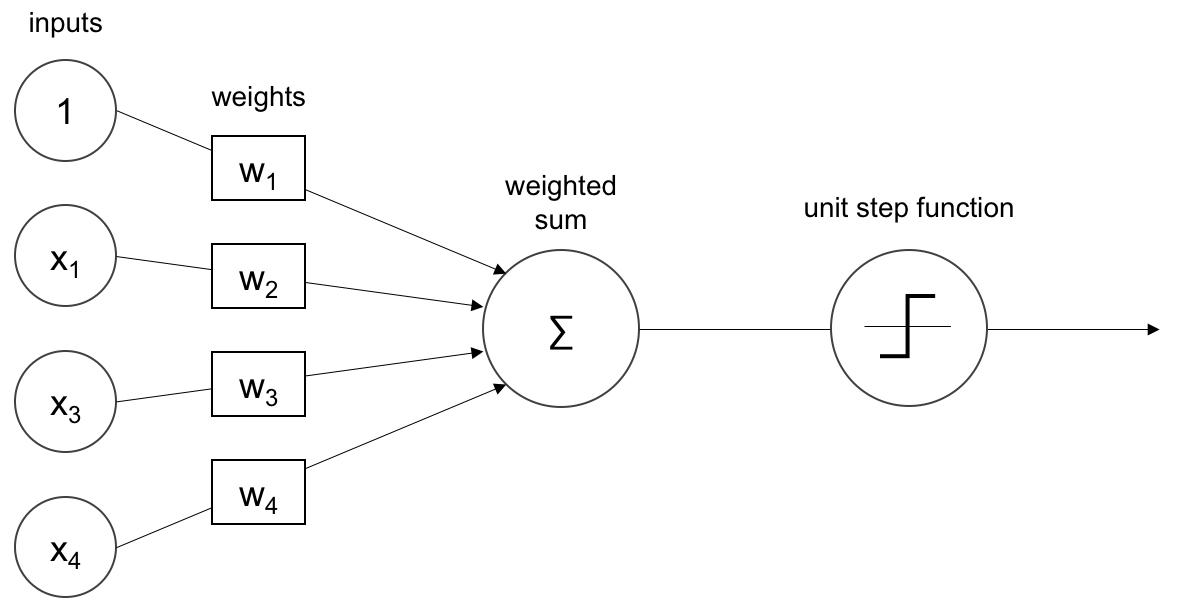
\includegraphics[width = 1 \textwidth]{Neural_Network/perceptron_schema.png}
            \caption{Schema of the Perceptron neuron}
        \end{center} 
    \end{minipage}
    \hspace{1em}
    \begin{minipage}{5cm}
        The Neural Network is made by individual neurons called \textit{Perceptrons}. The neurons are split into input, weights and activation functions.\\
        Nevertheless, the most important part of the neuron that determines significantly the capabilities of the neuron, is the activation function (which returns the output of the neuron).
    \end{minipage}
\end{figure}\\
The traditional activation function used in the Multilayer Perceptron is the Sigmoid: 
\begin{equation*}
f(x) = \cfrac{1}{1+e^{-w\cdot x}},\text{ where: } x,w\in\mathbb{R}^n
\end{equation*}
The Multilayer Perceptron Topology can be split into layers of three types:
\begin{figure}[h]
    \begin{minipage}{9cm}
        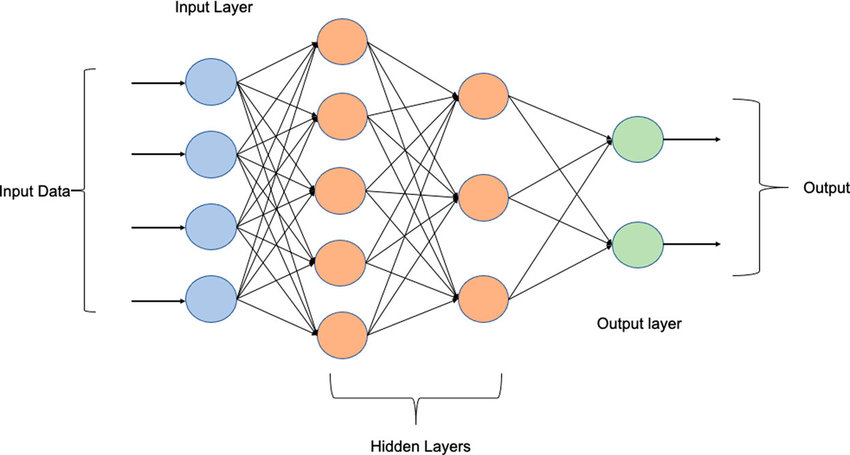
\includegraphics[width = 1 \textwidth]{Neural_Network/Multi-layer-perceptron-MLP-NN-basic-Architecture.png}
        \caption{Schema of the Multilayer perceptron}
    \end{minipage}
    \hspace{1em}
    \begin{minipage}{5cm}
        \begin{itemize}
            \item \textbf{Input Layer}: The initial set of neurons of the Multilayer Perceptron.
            \item \textbf{Output Layer}: The final set of neurons of the Multilayer Perceptron.
            \item \textbf{Hidden Layers}: The set of neurons (in layers) between the input and output layers.
        \end{itemize}
    \end{minipage}
\end{figure}\\
\newpage
\hspace{-1.6em}The training process uses the \textbf{BackPropagation}\footnote{The BackPropagation method and how it works can be consulted in the following \href{https://en.wikipedia.org/wiki/Backpropagation}{link}} method. 
The requirements of \textit{backpropagation} are the \textit{learning rate} (a parameter that determines how much the network will be modified while applying the method) and the \textit{optimization method} (an algorithm to reduce the network's \textit{error function}\footnote{The error function is introduced and explained on page \pageref{whyworks}.}).\\ 
The training process of neural networks is divided into \textit{epochs}, the number of iterations where \textit{backpropagation} is applied with a number of \textit{batches}. The \textit{batch} (or \textit{batch size}) is the number of samples used in every \textit{epoch}, and the \textit{mini batch} (or \textit{mini batch size}) is the number of samples used to apply the \textit{optimization method} (using this number of samples to create a mean modification of the parameters).\\ 
In this study, the \textit{mini batch} will be 1 and the \textit{batch size} will be the number of samples; that is to say, every \textit{epoch} will apply \textit{backpropagation} for every sample.\\ 
Moreover, the neural network will be implemented in \textbf{C language} to improve efficiency, with all methods (\textit{backpropagation}, \textit{optimization method}, \textit{error function}, etc.) developed by hand to ensure minimal computational cost.

% WHY WORKS
\subsection{Why Neural Networks work}
\label{whyworks}
It is important to remark that what gives us the capability to model any system is that we can express every problem as a function (no matter if it is a classification task, probability function, prediction, or regression function).\\
The association between a task and a function allow us to apply the \textbf{Universal Approximation Theorem}.\\
\rule{\linewidth}{0.4pt}
\begin{itemize}
    \item \textbf{Definition:} Universal Approximation Theorem.
\end{itemize}  
For any function $f:\mathbb{R}^n \rightarrow \mathbb{R}^m$, with $m,n\in\mathbb{N}$, and a subset $D\subset \mathbb{R}^n$ where $f$ is continuous at all $D$, 
$\exists \{(w_i, b_i, c_i)\}_{i = 0}^k$ that: 
$$f(\vec{x}) - \lim_{k \rightarrow \infty} \sum_{i=0}^{k} c_i \sigma \left( w_i^T \cdot \vec{x} + b_i \right) = 0$$
Where $w_i \in \mathbb{R}^n$, $b_i\in \mathbb{R}$, $c_i \in \mathbb{R}^m$, $\vec{x}\in D$ and $\sigma$ the sigmoid function.\\
\rule{\linewidth}{0.4pt}\\\vspace{0.5em}
The parameters $\{w_i, b_i, c_i\}$ are associated (respectively) with the weights, bias and scale factor of the i-th neuron.\\
Neural Networks essentially use this theorem with a limited number of sigmoids (equal to de number of neurons), consecuently an error of approximation is given.
$$f(\vec{x})-\sum_{i=0}^{k} c_i \sigma \left( w_i^T \cdot \vec{x} + b_i \right) = \epsilon, k \in \mathbb{N}$$
Modeling systems the information of the function shape/tendency is limited or none, making it only possible to study the problem using data values.\\
This cases are handle using the \textit{square-norm} metric (or \textit{Mean Squared Error}).\\
\newpage
\hspace{-1.6em}\rule{\linewidth}{0.4pt}
\begin{itemize}
    \item \textbf{Definition:} Square-norm: 
\end{itemize}
Being $f:\mathbb{R}^n \rightarrow \mathbb{R}^m$ function followed by the system.
Being $g:\mathbb{R}^n \rightarrow \mathbb{R}^m$, with $m,n\in\mathbb{N}$, as $g(\vec{x}) = \sum_{i=0}^{k} c_i \sigma \left( w_i^T \cdot \vec{x} + b_i \right)$, $k\in\mathbb{N}$.\\
Given a dataset $B = \{(\vec{x_i},\vec{y_i})\}_{i=0}^{N}$, with $N \in \mathbb{N}$, where $\forall (\vec{x_i},\vec{y_i}) \in B, \vec{y_i} = f(\vec{x_i})$.
$$\Delta^2 = \frac{1}{N} \sum_{i=0}^{N} \left( \vec{y_i} - g(\vec{x_i}) \right)^2$$
\rule{\linewidth}{0.4pt}\\\vspace{0.5em}
Decreassing the error $\Delta$ implies reducing the error $\epsilon$ because as $\Delta$ decrease the model improves its approximation.\\
As more neurons are added to the Network, the approximation and the training time increases. This increase in training time may not be worth as it can represent a minimum improvement of the model.\\
Moreover, the Backpropagation\footnote{The Backpropagation method is an algorithm to modify the internal parameters of a Neural network by using the chain rule, more information in the following \href{https://en.wikipedia.org/wiki/Backpropagation}{link}.} method used to train Neural Networks have a complexity that increases the processing time exponentially to the number of neurons.\\
Therefore, trying to obtain the ideal topology for solving a problem is a difficult task that in many cases resides in trial and error.

\section{Neural Networks topology}
The main objective of the study is to obtain a more efficient process using neural networks than the traditional ways that have been used to date.\\
As it has been explained before, there is not an understanable process through which to obtain an efficient neural network.\\
While approaching this problem, an idea that could partially solve the lack of understanding of what the neural network is doing, and deduce the optimal architecture, came to mind. 
\subsection{Hypotesis and Working Hypothesis}
As it has been said before, when approaching this problem an intuitive idea appeared. \\
\rule{\linewidth}{0.4pt}
\begin{itemize}
    \item \textbf{Working Hypothesis:} If there is enough information about the system to model, there exists an efficient neural network whose architecture can be obtained using rules.
\end{itemize}
\rule{\linewidth}{0.4pt}\\ \vspace{0.5em}
The idea proposed is influenced by the following observations:
\begin{enumerate}
    \item Every deterministic process is a combination of restrictions that can be represented as a function.
    \item Every function can be split into domains its behaviour can be categorized as periodical, irrational, or polynomial.
    \item The periodical, polynomial and irrational functions are continuous in "all"\footnote{In case of irrational functions such as $\sqrt{x}$, it can be interpreted as $f(x) = \left\{ \begin{matrix} 0, x < 0 \\ \sqrt(x), x \geq 0 \end{matrix} \right.$} domain.
    \item All continuous functions can be approximated using the \textbf{Universal Approximation Theorem}.
\end{enumerate}
Moreover, if a function does not follow one of these types of functions, it can be split by more intervals until each of them can be approximated by one of these types or even can be approximated using \textit{Fourier Series} or \textit{Taylor series} allowing it to be modelled by periodical and polynomial functions.\\
Therefore, this Working Hypothesis can be verified by reducing it to corroborate the following points:
\begin{enumerate}
    \item Each category of functions mentioned can be modelled using a particular architecture of a neural network.
    \item There is a determined minimum number of data registers where the neural network can be trained.  
\end{enumerate}
To verify the Working Hypothesis, efficiency and precision studies are required.

\subsection{Study of deterministic processes}
To start, let's assume the following axioms to simplify the study and give some feedback to make the correlations to verify or dismiss the Working Hypothesis.
\begin{enumerate}
    \item All periodic functions can be approximated as a combination of $\sin$ functions.
    \item All polynomial functions can be approximated as a combination of $x^n$ functions, where $n\in \{\mathbb{N} \cup \{0\}\}$.
    \item All \underline{irrational functions}\footnote{In this study, \textit{irrational functions} define the functions that present an n-th root.} can be approximated as a combination of $\sqrt{x}$ function.
\end{enumerate} 
All points can be proven using \textit{Taylor Series} and \textit{Fourier Series}.
The study will be reduced to taking patterns of the architectures used to approximate the functions $\sin{x}, \sqrt{x}, x^2$.\\
This paper uses $I-H-N-O$ nomenclature to represent the architecture of the neural network, where the letters $I,H,N,O$ represent the number of inputs, the hidden layers, the number of neurons for each hidden layer and the number of outputs respectively.\\
For instance, the architecture $1-3-4-1$ is a network with 1 input, 3 hidden layers with 4 neurons each one and 1 output.

\subsubsection{Study of the \textit{sin} function}
To test if there exists an architecture that can approximate efficiently the $\sin$ function in the real plane, the approximation of the function is studied in the interval $[0, 2\pi]$ using a fixed number of iterations with different architectures.
\begin{figure}[h]
    \centering
    \subfloat[Model 1-1-1-1]{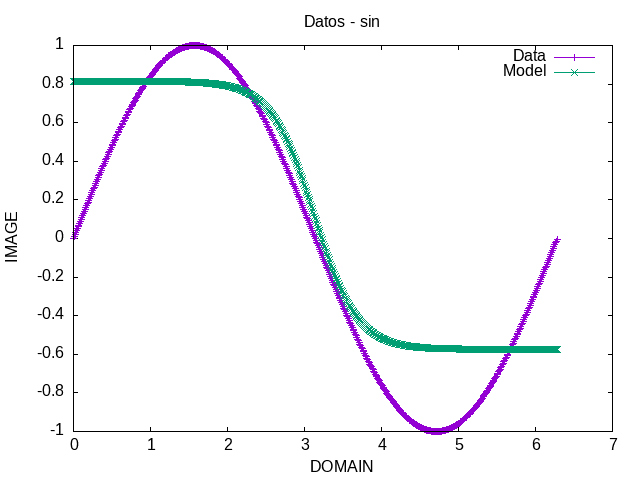
\includegraphics[width=0.24\linewidth]{img/sin/sin-1-1-1-1.png}}
    \subfloat[MSE 1-1-1-1]{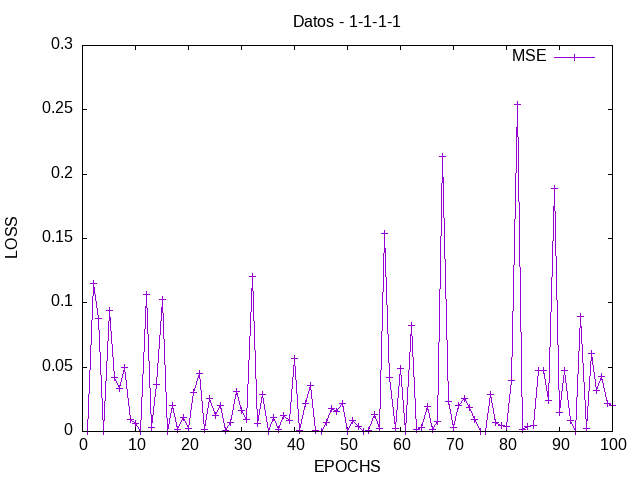
\includegraphics[width=0.24\linewidth]{img/sin/sin-loss-1-1-1-1.png}}
    \hspace{1em}
    \subfloat[Model 1-1-2-1]{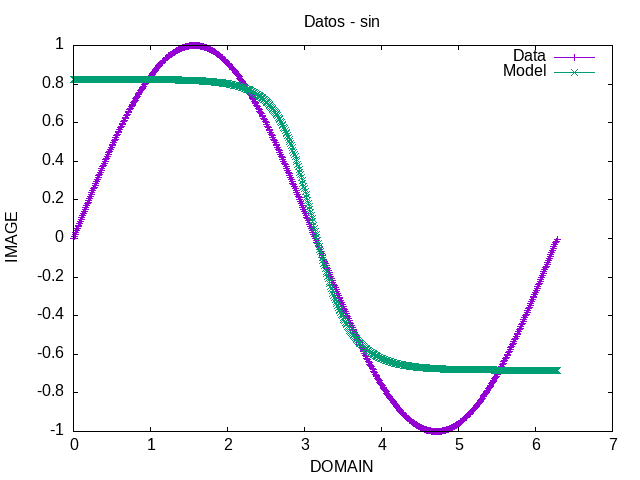
\includegraphics[width=0.24\linewidth]{img/sin/sin-1-1-2-1.png}}
    \subfloat[MSE 1-1-2-1]{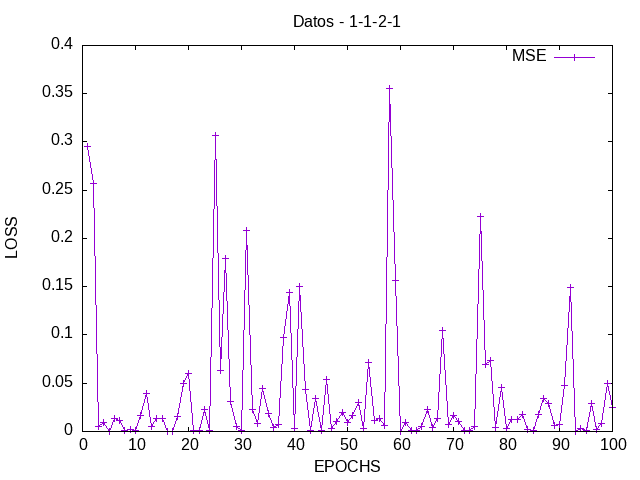
\includegraphics[width=0.24\linewidth]{img/sin/sin-loss-1-1-2-1.png}}
    \\
    \subfloat[Model 1-1-3-1]{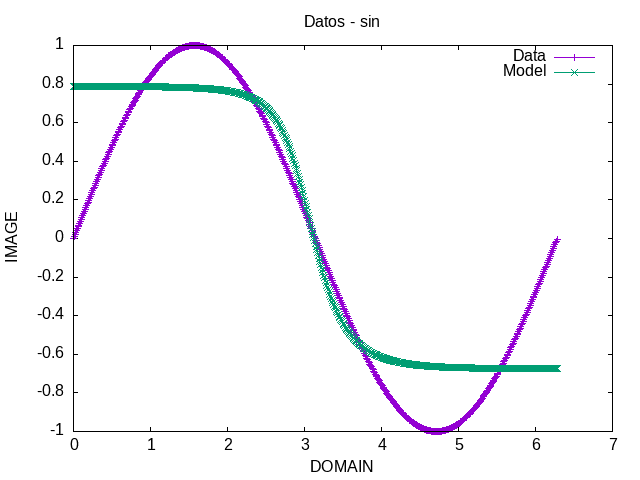
\includegraphics[width=0.24\linewidth]{img/sin/sin-1-1-3-1.png}} 
    \subfloat[MSE 1-1-3-1]{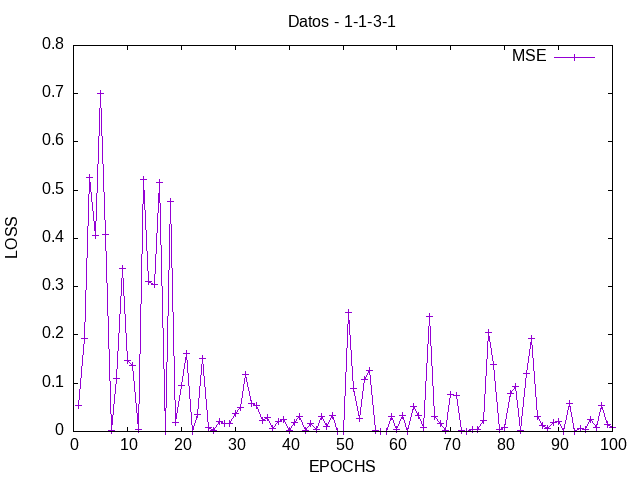
\includegraphics[width=0.24\linewidth]{img/sin/sin-loss-1-1-3-1.png}}
    \hspace{1em}
    \subfloat[Model 1-2-2-1]{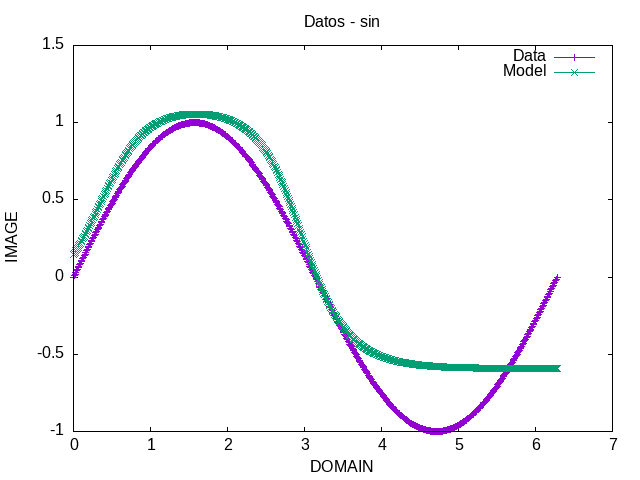
\includegraphics[width=0.24\linewidth]{img/sin/sin-1-2-2-1.png}}
    \subfloat[MSE 1-2-2-1]{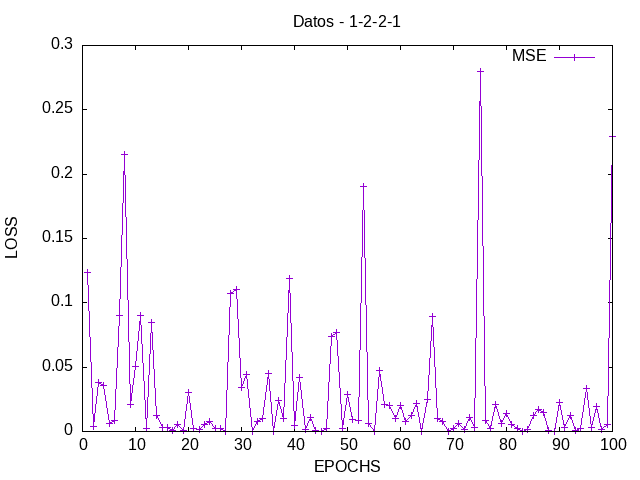
\includegraphics[width=0.24\linewidth]{img/sin/sin-loss-1-2-2-1.png}}
    \\
    \subfloat[Model 1-2-4-1]{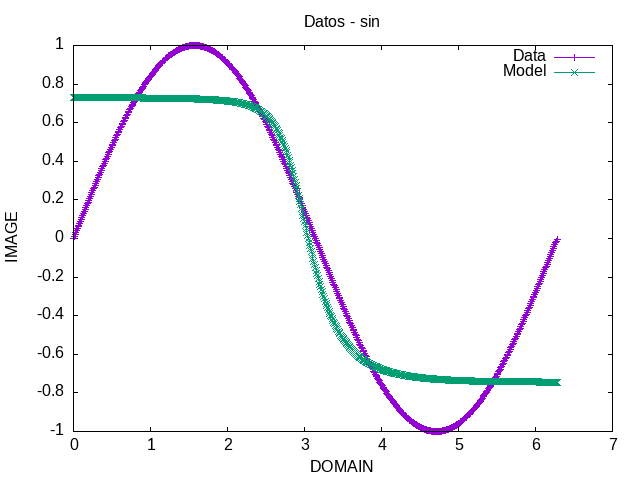
\includegraphics[width=0.24\linewidth]{img/sin/sin-1-2-4-1.png}}
    \subfloat[MSE 1-2-4-1]{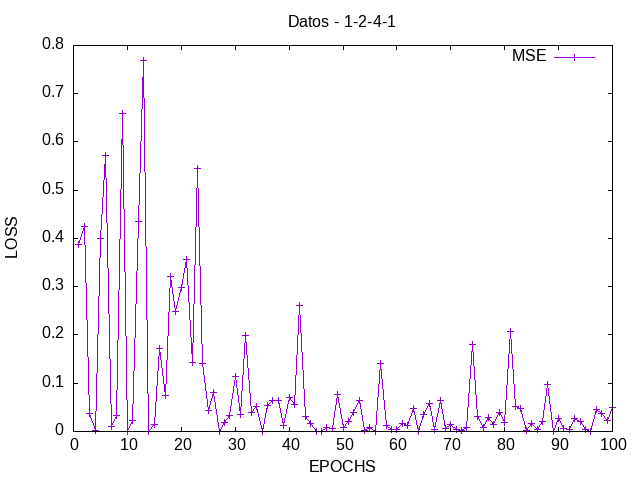
\includegraphics[width=0.24\linewidth]{img/sin/sin-loss-1-2-4-1.png}}
    \hspace{1em}
    \subfloat[Model 1-4-2-1]{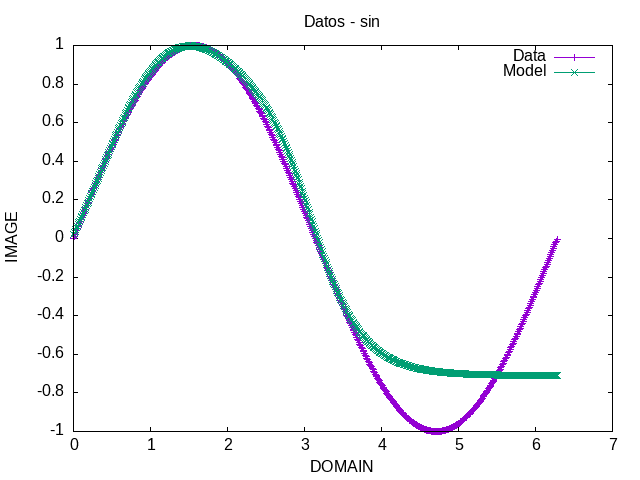
\includegraphics[width=0.24\linewidth]{img/sin/sin-1-4-2-1.png}}
    \subfloat[MSE 1-4-2-1]{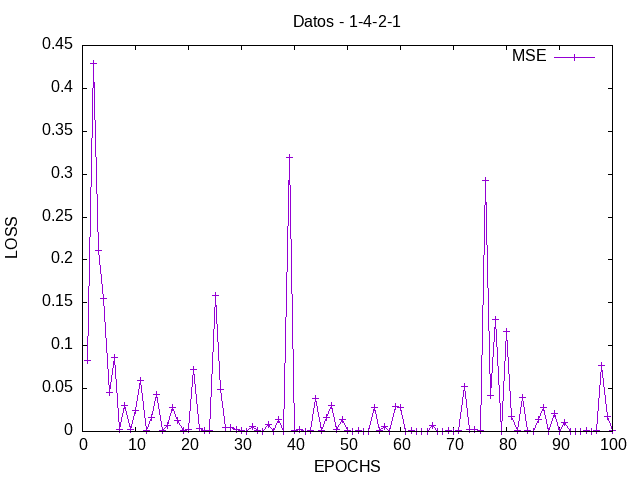
\includegraphics[width=0.24\linewidth]{img/sin/sin-loss-1-4-2-1.png}}
    \caption{Results of different architectures approximating the function \textit{sin}}
    \label{fsin100}
\end{figure}\\
The results shown in Figure \ref{fsin100} were obtained 
by fixing 100 epochs and training the networks using the \textit{Stochastic Gradient Descent} method with a learning rate of $0.1$ trying to minimize the \textit{Square-norm} error (\textit{MSE}).\\
\newpage
\hspace{-1.6em}As can be seen in the Figure, almost all architectures do not approximate the $\sin$ function properly, not counting the architectures \textit{1-2-2-1} and \textit{1-4-2-1} which approximates the function relatively correctly.\\
If the experiment is repeated changing the epoch number (instead of 100 change to 200) the results are almost similar (with more precision in some parts but no improvement of modelation).\\
However, the architectures \textit{1-4-4-1} and \textit{1-4-2-1} give an augment of precision significantly rellevant.
\begin{figure}[h]
    \subfloat[Model 1-4-2-1]{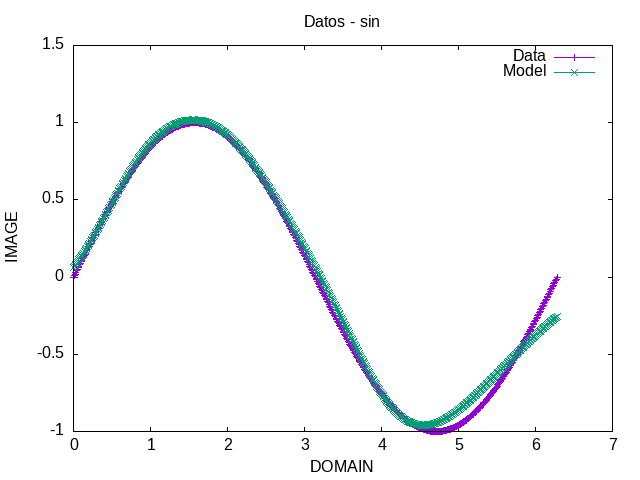
\includegraphics[width=0.24\linewidth]{img/sin/sin-1-4-2-1(200).png}}
    \subfloat[MSE 1-4-2-1]{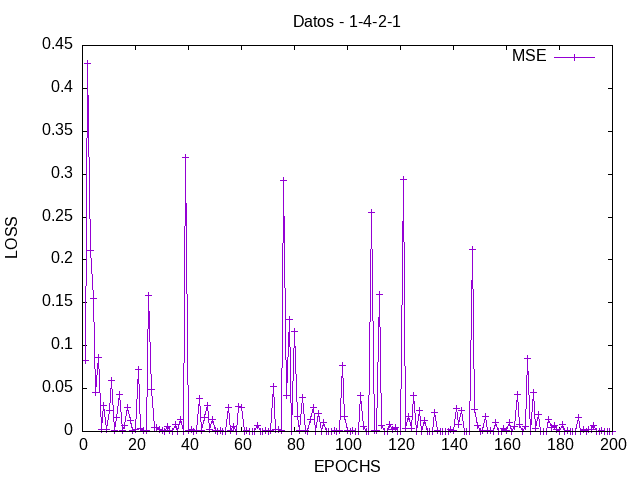
\includegraphics[width=0.24\linewidth]{img/sin/sin-loss-1-4-2-1(200).png}}
    \hspace{1em}
    \subfloat[Model 1-4-4-1]{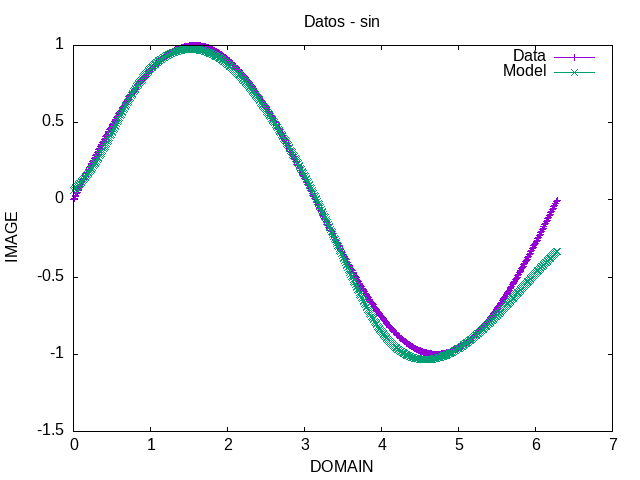
\includegraphics[width=0.24\linewidth]{img/sin/sin-1-4-4-1(200).png}}
    \subfloat[MSE 1-4-4-1]{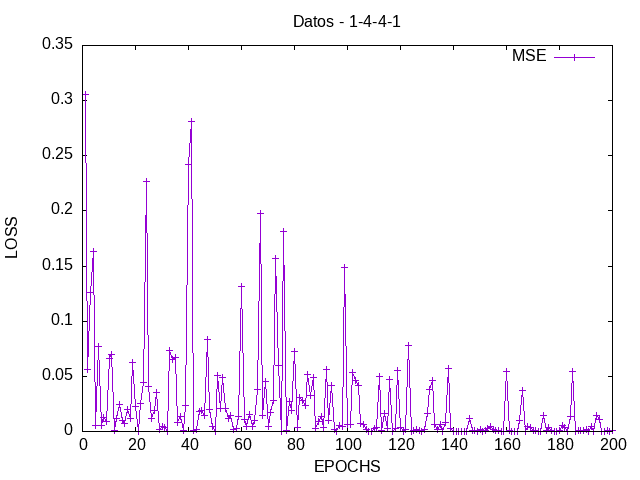
\includegraphics[width=0.24\linewidth]{img/sin/sin-loss-1-4-4-1(200).png}}
    \caption{Architectures that improves the modelisation of \textit{sin} function}
    \label{fsin200}
\end{figure}\\
The approximation done by these architectures is so significant that allows us to observe and conclude that the model that approximates the best the $\sin$ function is $1-2-4-1$.\\
\newpage
\hspace{-1.6em}The following conclusion is obtained because this is an architecture that efficiently approximates the function it aims to "learn"\footnote{Learn in this term refers as if the training process allows to reduce the loss (also named error) near 0 with a significant decrease throughout the epochs.}.\\
Moreover, it can be an evidence of the following idea:\\
\rule{\linewidth}{0.4pt}
\begin{itemize}
    \item \textbf{Suggested Hypotesis:} To approximate any periodical function in a real plane a minimum of 2 neurons is needed in each of the $K$ hidden layers, where $K$ is the sum of the relative extremes and points of inflexion of the function.
\end{itemize}
\rule{\linewidth}{0.4pt}\\ \vspace{0.5em}
This suggestion is obtained by the intuition and observation that every layer of the neural network could be modelling one interval (delimited by the extremes of the function and inflexion points) and performing that approximation seems to need at least 2 sigmoids.

\subsubsection{Study of the \textit{parabolic} function}
The same experiment has been done with the function $x^2$ (also with function $x^3$ to have more results to compare) with fixed epochs, learning rate and domain.\\
Specifically, the values of epochs, learning rate and domain used are, respectively, $100$, $0.1$ and $[-2,2]$.\\
The results obtained for polynomial functions are shown in \ref{poli100}.
\begin{figure}[h!]
    \centering
    \subfloat[\centering Model\\1-1-1-1]{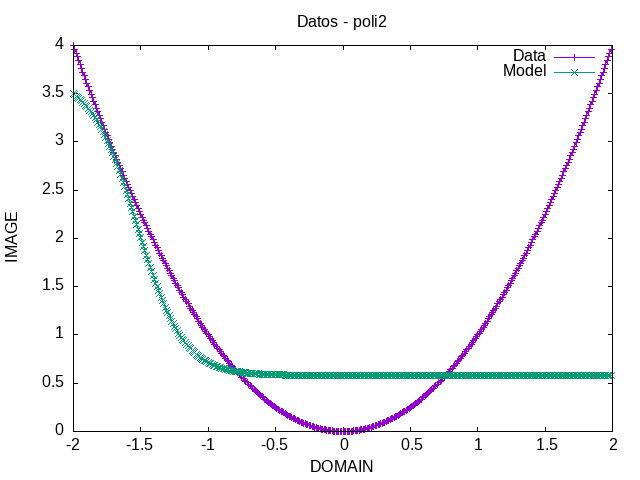
\includegraphics[width=0.15\linewidth]{img/poli/poli2-1-1-1-1.png}}
    \subfloat[\centering MSE\\1-1-1-1]{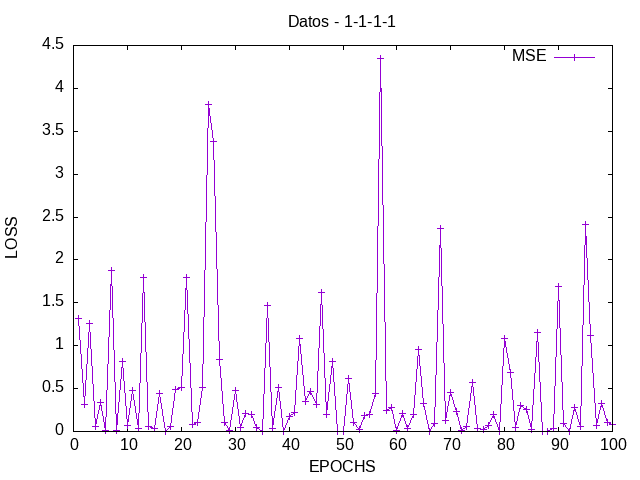
\includegraphics[width=0.15\linewidth]{img/poli/poli2-loss-1-1-1-1.png}} \hspace{0.5em}
    \subfloat[\centering Model\\1-2-1-1]{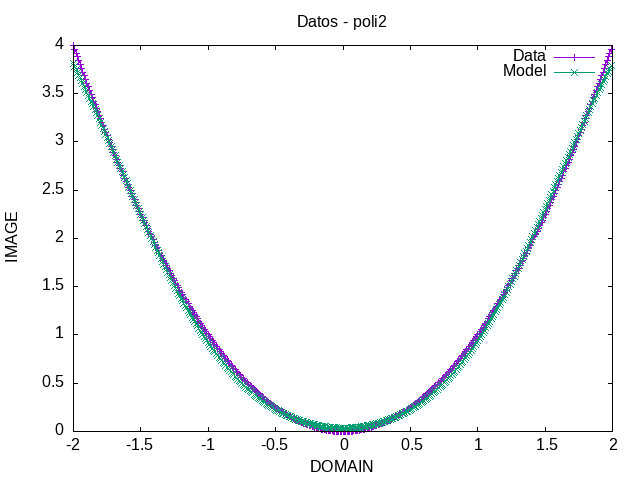
\includegraphics[width=0.15\linewidth]{img/poli/poli2-1-2-1-1.png}}
    \subfloat[\centering MSE\\1-2-1-1]{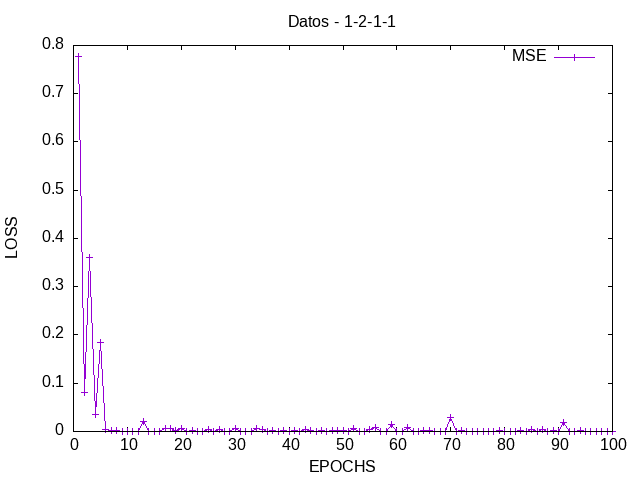
\includegraphics[width=0.15\linewidth]{img/poli/poli2-loss-1-2-1-1.png}} \hspace{0.5em}
    \subfloat[\centering Model\\1-2-2-1]{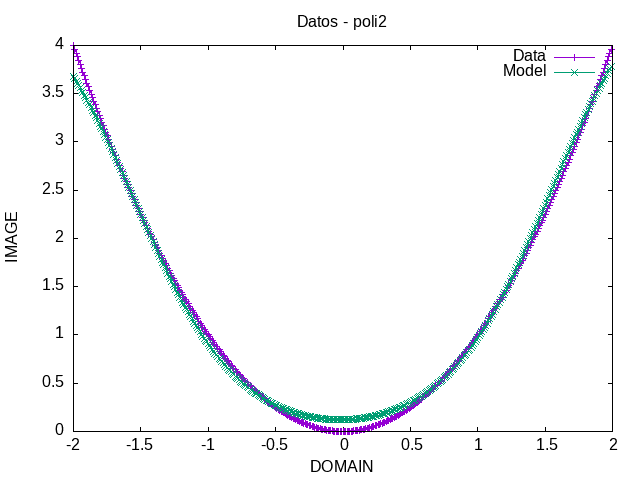
\includegraphics[width=0.15\linewidth]{img/poli/poli2-1-2-2-1.png}}
    \subfloat[\centering MSE\\1-2-2-1]{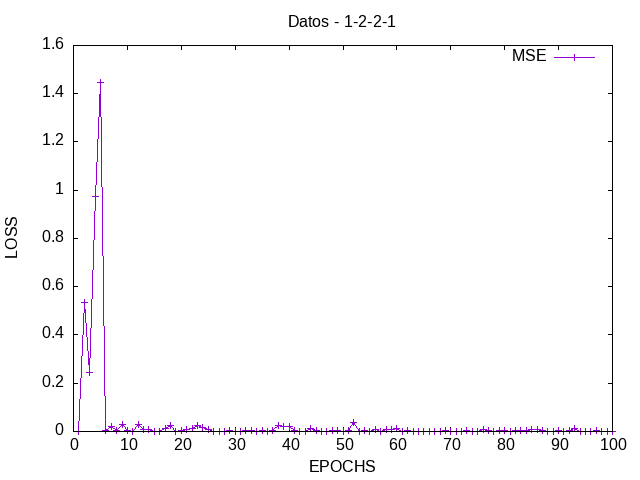
\includegraphics[width=0.15\linewidth]{img/poli/poli2-loss-1-2-2-1.png}}
    \\\vspace{1em}
    \subfloat[\centering Model\\1-1-1-1]{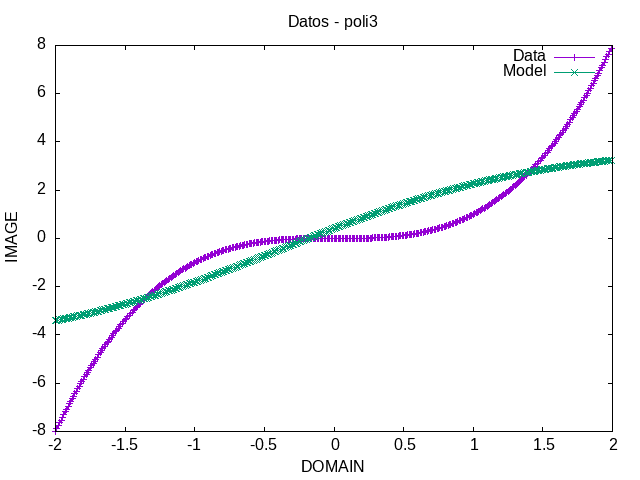
\includegraphics[width=0.15\linewidth]{img/poli/poli3-1-1-1-1.png}}
    \subfloat[\centering MSE\\1-1-1-1]{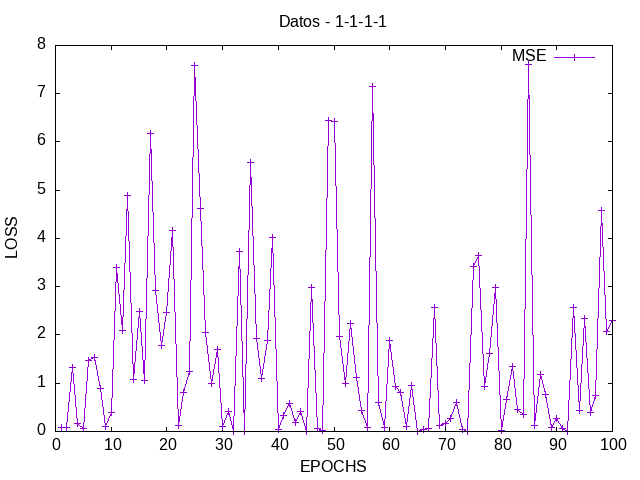
\includegraphics[width=0.15\linewidth]{img/poli/poli3-loss-1-1-1-1.png}} \hspace{0.5em}
    \subfloat[\centering Model\\1-2-1-1]{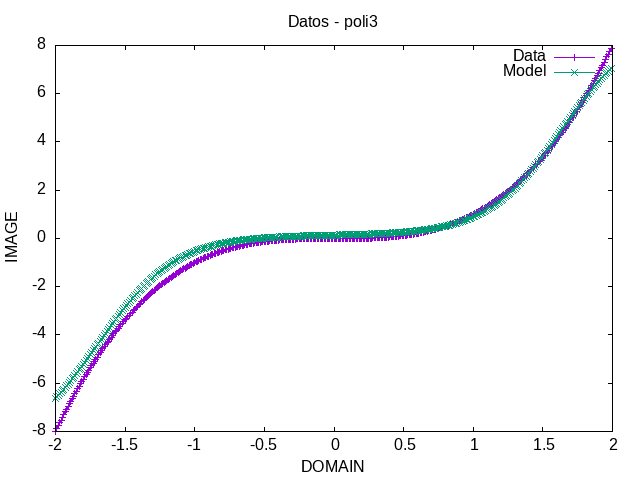
\includegraphics[width=0.15\linewidth]{img/poli/poli3-1-2-1-1.png}}
    \subfloat[\centering MSE\\1-2-1-1]{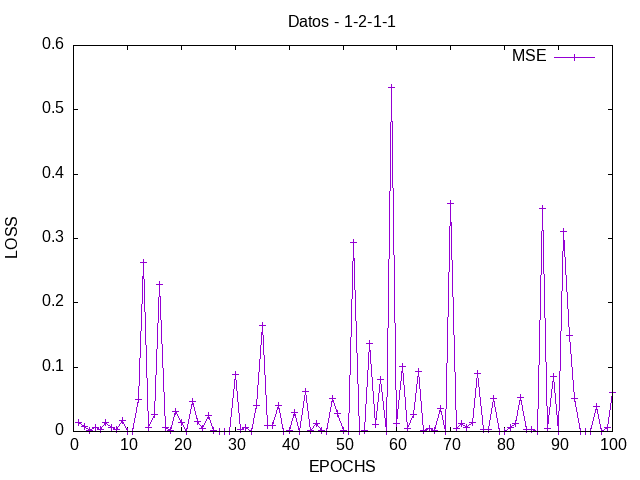
\includegraphics[width=0.15\linewidth]{img/poli/poli3-loss-1-2-1-1.png}} \hspace{0.5em}
    \subfloat[\centering Model\\1-2-2-1]{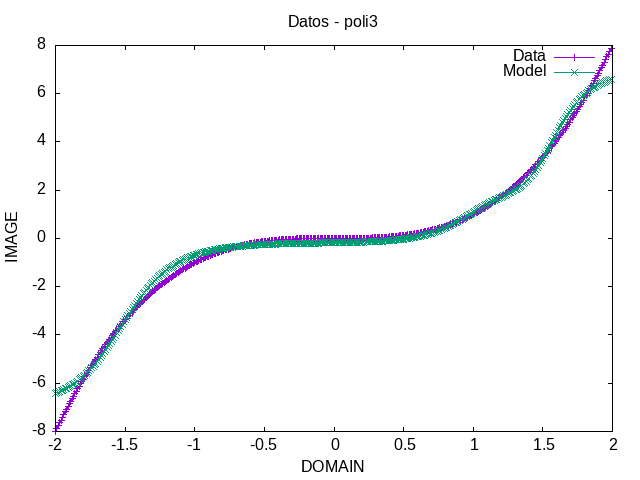
\includegraphics[width=0.15\linewidth]{img/poli/poli3-1-2-2-1.png}}
    \subfloat[\centering MSE\\1-2-2-1]{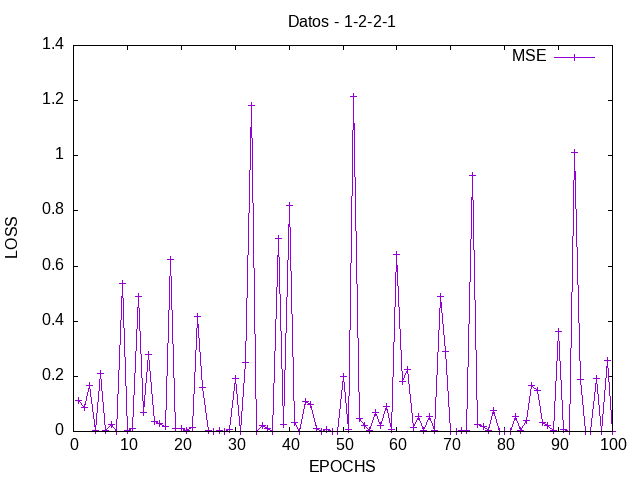
\includegraphics[width=0.15\linewidth]{img/poli/poli3-loss-1-2-2-1.png}}
    \caption{Results of different architectures approximating the functions $x^2$ and $x^3$}
    \label{poli100}
\end{figure}\\
It shows how the most efficient architecture, which gives the better performance in modelling and precision, is the $1-2-1-1$.\\
This architecture was tested before with the periodical functions but without possitive results. However, in this case is the best, which was one of the axioms proposed, each type of function has a diferent optimal architecture.\\
Therefore, a last study will be done to obtain the architecture needed to model the irrational functions.
\newpage

\subsubsection{Study of the \textit{squared root} function}
Finally, reproducing the experiment for the function $\sqrt{x}$, the results obtained are shown in \ref{sqrt100}.
\begin{figure}[h]
    \centering
    \subfloat[Model 1-1-1-1]{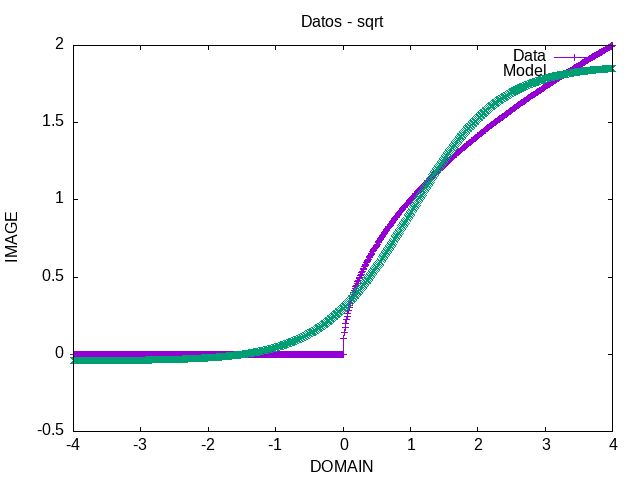
\includegraphics[width=0.24\linewidth]{img/sqrt/sqrt-1-1-1-1.png}}
    \subfloat[MSE 1-1-1-1]{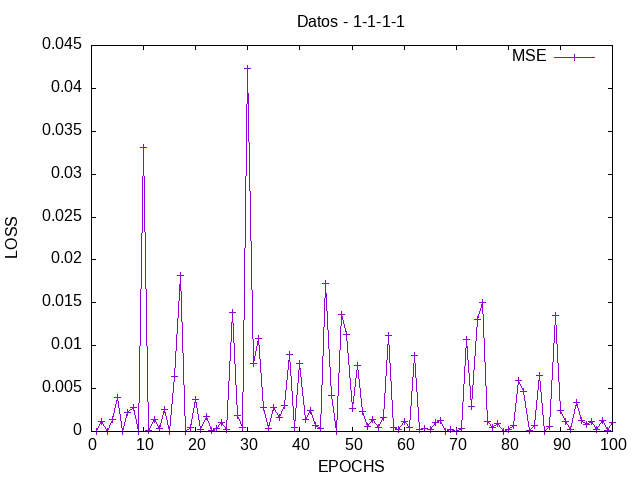
\includegraphics[width=0.24\linewidth]{img/sqrt/sqrt-loss-1-1-1-1.png}}
    \hspace{1em}
    \subfloat[Model 1-1-2-1]{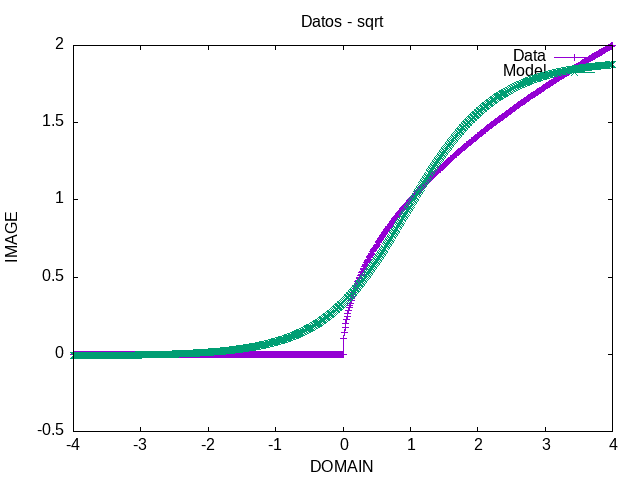
\includegraphics[width=0.24\linewidth]{img/sqrt/sqrt-1-1-2-1.png}}
    \subfloat[MSE 1-1-2-1]{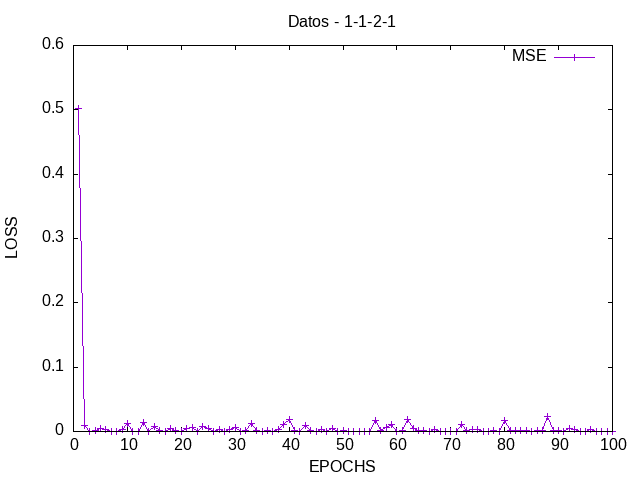
\includegraphics[width=0.24\linewidth]{img/sqrt/sqrt-loss-1-1-2-1.png}}
    \\
    \subfloat[Model 1-2-1-1]{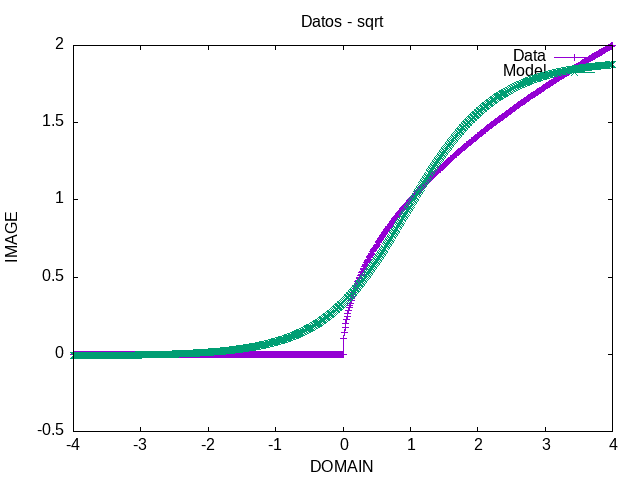
\includegraphics[width=0.24\linewidth]{img/sqrt/sqrt-1-2-1-1.png}} 
    \subfloat[MSE 1-2-1-1]{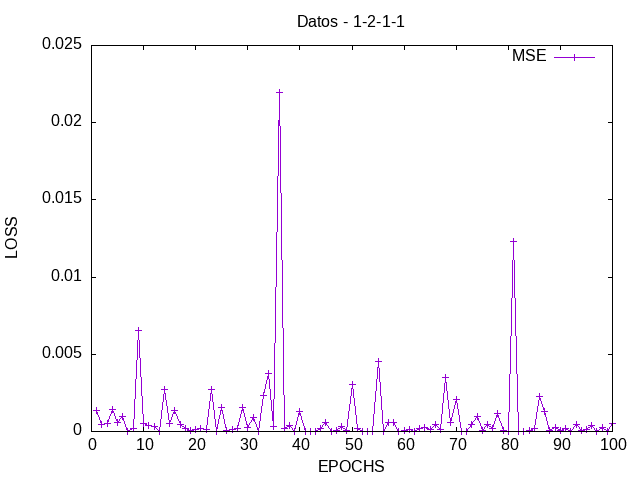
\includegraphics[width=0.24\linewidth]{img/sqrt/sqrt-loss-1-2-1-1.png}}
    \hspace{1em}
    \subfloat[Model 1-3-1-1]{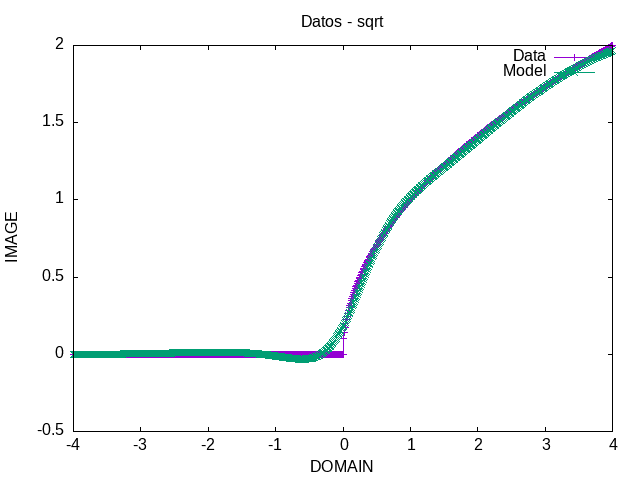
\includegraphics[width=0.24\linewidth]{img/sqrt/sqrt-1-3-1-1.png}}
    \subfloat[MSE 1-3-1-1]{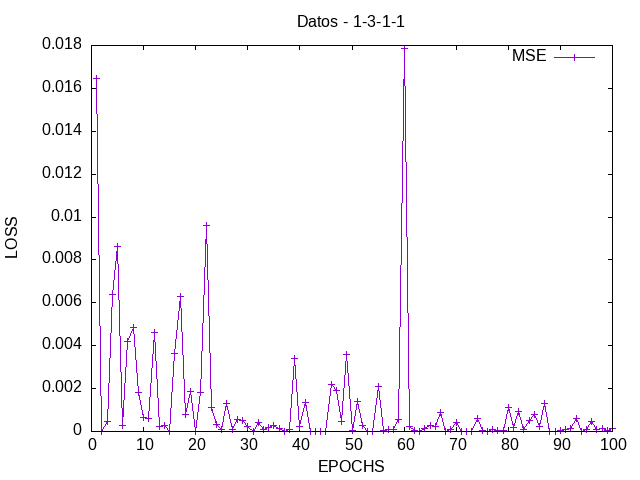
\includegraphics[width=0.24\linewidth]{img/sqrt/sqrt-loss-1-3-1-1.png}}
    \caption{Results of different architectures approximating the function $\sqrt{x}$}
    \label{sqrt100}
\end{figure}\\
In this study, the only parameter that was changed with respect to the previous experiments was the domain (which was increased to the interval $[-4,4]$).\\
As it can be observed, the architecture that approximates the best the function is $1-3-1-1$.\\
Furthermore, it should also be commented that the intuition of the inclusion of irrational functions such as the $\sqrt{x}$ in the axioms of the Working Hypothesis was made to use the property of having a function similar to $ReLU$\footnote{The \textit{ReLU} function is widely used as an activation function which is defined as $f(x) = \left\{ \begin{matrix} 0, x < 0 \\ x, x\geq 0\end{matrix} \right.$}.\\

\subsection{Viability of approximation discontinuous functions}
It is important to keep in mind that splitting functions into domains can develop in discontinuities which do not allow the use of the \textbf{Universal Approximation Theorem}.\\
Nevertheless, the application of neural networks in tasks such as classification or regression in many areas, with no information of the function that is approximating, using activation functions different from the \textit{sigmoid} that give (apparently) correct results give the idea that possibly the theorem could be expanded and (in some cases) have no need of the continuity restriction.\\
The widely use of $ReLU$ function in neural networks is because it is easier to program and with enough neurons, its effects (depite it should not be possible) give a similar or even better results.\\
\newpage
\hspace{-1.6em}\rule{\linewidth}{0.4pt}
\begin{itemize}
    \item \textbf{Suggested Hypotesis:} If a function has discontinuities different from asymptotic, the \textbf{Universal Approximation Theorem} can be used to give an approximation with error 0 when the number of sigmoid tends to infinity.
\end{itemize}
\rule{\linewidth}{0.4pt}\\ \vspace{0.5em}
This Suggested Hypothesis can be sustained by the ability of sigmoid functions to approximate jump discontinuities. However, an experiment with discontinuous functions has been done to give evidence for this hypothesis.
\subsubsection{Study of Jump discontinuity}
In this experiment, a simple architecture of $1-2-2-1$ with a high amount of epochs (concretely $10000$) and fixed learning rate of $0.1$ have been used to approximate the function:
$$ f(x) = \left\{ \begin{matrix}
    1, x \leq 1 \\
    0, x \in (1,2] \\
 -1, x > 2
\end{matrix} \right. $$
The results of approximating the function in the interval $[0,3]$ are shown in \ref{disc}.
\begin{figure}[h]
    \centering
    \subfloat[Model]{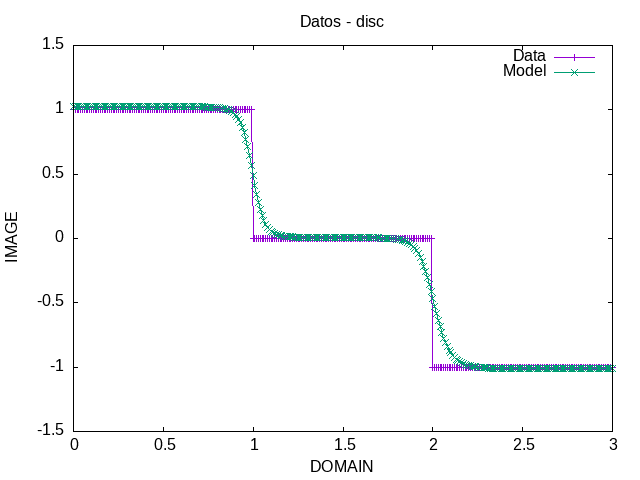
\includegraphics[width=0.5\linewidth]{img/disc/disc-1-2-2-1.png}}
    \subfloat[MSE]{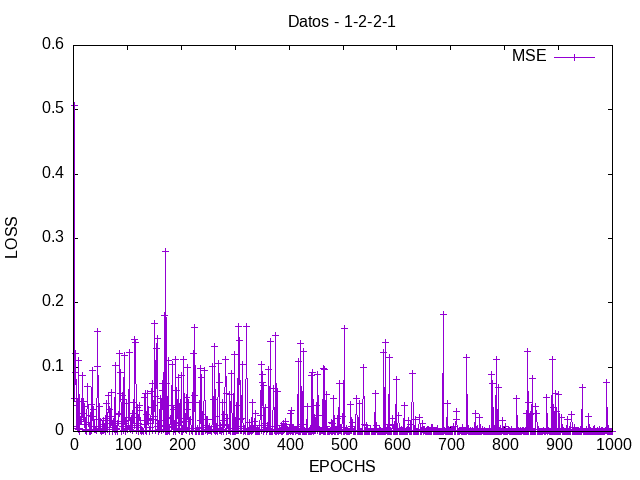
\includegraphics[width=0.5\linewidth]{img/disc/disc-loss-1-2-2-1.png}}
    \caption{Architecture $1-2-2-1$ approximation to a jump discontinuity function}
    \label{disc}
\end{figure}\\
As can be seen in the figure \ref{disc}, using a limited model with enough number of epochs the approximation is quite acceptable. Therefore the use of \textit{sigmoid} functions in approximate split functions with jump discontinuities can be used at least in some cases.

\subsubsection{Study of Asimptotyc discontinuity}
However, the application of the \textbf{Universal Approximation Theorem} in discontinuities such as asymptotic can cause problems that avert the modelation using sigmoids.\\
Repeating the experiment done with the jump discontinuity function, but with a more powerful architecture, to approximate the function $\tan{x}$ in the interval $[-\frac{\pi}{2},\frac{\pi}{2}]$ give us an idea of this problem.\\
The results obtained are shown in \ref{asymp}.
\begin{figure}[h]
    \centering
    \subfloat[Model]{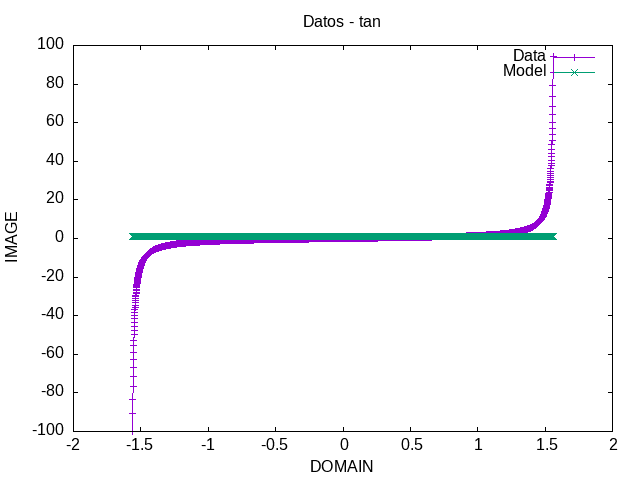
\includegraphics[width=0.5\linewidth]{img/disc/tan-1-5-5-1.png}}
    \subfloat[MSE]{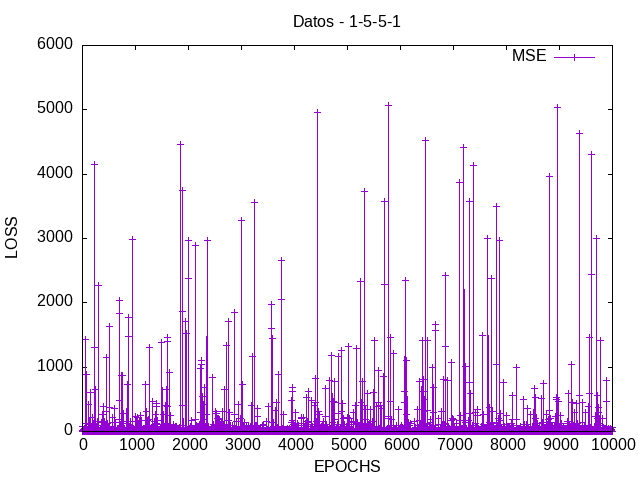
\includegraphics[width=0.5\linewidth]{img/disc/tan-loss-1-5-5-1.png}}
    \caption{Architecture $1-5-5-1$ approximation to $\tan{x}$ function}
    \label{asymp}
\end{figure}\\
\newpage
\hspace{-1.6em}As can be observed the neural network is limited and cannot approximate properly the function. However, the use of other activation functions such as the $ReLU$ mentioned before can give a better performance.\\
In the case of using the $ReLU$ function, it gives another problem that can be difficult to handle, the \textbf{Universal Approximation Theorem} does not ensure that the resulting function approximates the system with a limited error.\\
Moreover, the use of the \textit{BackPropagation} method and its dependency with the \textit{Newtons Method} (the \textit{Steepest Gradient Descend}) to obtain zeros of the \textit{cost function} in the training process, does not ensure that the solution it arrives is the best or, even though, if it is correct in all cases (and we can be blind in situations were the network was not tested).\\

\subsection{Observations of the results}
To sum up, all the results and conclusions obtained in the studies we can conclude if there is enough evidence for the initial working hypothesis.\\
\rule{\linewidth}{0.4pt}
\begin{itemize}
    \item \textbf{Working Hypothesis:} If there is enough information about the system to model,
    there exists an efficient neural network whose architecture can be obtained using
    rules.
\end{itemize}
\rule{\linewidth}{0.4pt}\\ \vspace{0.5em}
To verify the viability of the Working Hypothesis needed to accomplish the following conditions:
\newpage
\begin{enumerate}
    \item \underline{All periodic functions can be approximated as a combination of $\sin$ functions.}\vspace{0.5em}\\
 The first condition can be proven using \textit{Fourier series}\\
 However, it is important to mention that a periodical function such as $\tan{x}$ can not be approximated due to the asymptotes. \\
    \item \underline{All polynomial functions can be approximated as a combination of $x^n$ functions,}\\
    \underline{where $n\in \{\mathbb{N} \cup \{0\}\}$}.\vspace{0.5em}\\
 Such as the first condition, the second one can be proven using \textit{Taylor Series}, not having any inconvinient.\\
    \item \underline{All irrational functions can be approximated as a combination of the irrational}\\
    \underline{functions $\sqrt{x}$}.\vspace{0.5em}\\
 Point 3 can be explained by trying to approximate a function in a certain interval. Therefore it can be obtained the following deduction:\\
    \rule{\linewidth}{0.4pt}
    \begin{itemize}
        \item \textbf{Deduction:} Approximation of irrational functions.\\
 Being $f_n:\mathbb{R}\rightarrow\mathbb{R}$, $g:\mathbb{R}\rightarrow\mathbb{R}$ where $f_n(x) = \sqrt[n]{x}, \forall n \in \mathbb{N} / n > 1$ and $g(x) = \sqrt{x}$.\\
        $$ \exists c,d \in \mathbb{R} / \forall x \in [a,b], f_n(x)- g(c\cdot x + d) < \epsilon$$ 
 Where $\epsilon\in\mathbb{R^+}$ is the error and $\{ c,d \}$ are parameters that ajust $g$ to approximate $f_n$ in the interval $[a,b]\cup \mathbb{R}$.
    \end{itemize}
    \rule{\linewidth}{0.4pt}\\
 Nevertheless, mention that when $n$ (the degree of the root) is even the interval needs to be in the set $\mathbb{R^+}$. Moreover, this deduction can handle situations where the set of functions $f_n$ are defined as $f_n(x) = \alpha \sqrt[n]{x} + \beta$ where the parameters $\alpha,\beta \in \mathbb{R}$ \\
 This deduction can also be demonstrated using tangency:\\
    \rule{\linewidth}{0.4pt}
    \begin{itemize}
        \item \textbf{Proof:} Approximation of irrational functions.\\
 Being $f_n:\mathbb{R}\rightarrow\mathbb{R}$, $g:\mathbb{R}\rightarrow\mathbb{R}$ where $f_n(x) = \sqrt[n]{x}, \forall n \in \mathbb{N} / n > 1$ and $g(x) = \sqrt{x}$.\\
 Being $P=(p_0, p_1)\in[a,b]\subset \mathbb{R} / p_0 = \frac{a+b}{2}, p_1 = f_n(p_0)$, \\$\exists c,d\in\mathbb{R} / g(c\cdot p_0 + d) = p_1$.
 Therefore, 
        $$\exists (\alpha, \beta) \subset [a,b] / p_0 = \frac{\alpha + \beta}{2} \text{ where } \forall x \in (\alpha, \beta), |f_n(x) - g(c\cdot x + d)| < \epsilon$$
        $\epsilon\in\mathbb{R^+}$ the error.
    \end{itemize}
    \rule{\linewidth}{0.4pt}\\
 These demonstrations could be used for every function, not limiting them only to irrational functions.
\end{enumerate}
\begin{enumerate}
    \setcounter{enumi}{3}
    \item \underline{The mentioned functions can be modelled using a particular minimal and}\\
    \underline{distinguishable architecture.}\vspace{0.5em}\\
 The studies about the different architectures of the different functions ($x^2, \sin{x}, \sqrt{x}$) show that there exists a distinguishable minimum architecture that approximates the best of each function.\\
    \item \underline{There is a determined minimum number of data to train the neural network.}\vspace{0.5em}\\
 That point is controversial\footnote{It is controversial because the number of samples depends on the range of the interval and the backpropagation requires to perform good adjustments}. In all the studies the number of data available were different with at least $600$ registers. However, the relevant part about this is that it really needs a deterministic process that generates the dataset.\\
 The minimal information that is required is the deterministic process intrinsically. If there is no deterministic process the information needed will not be enough despite how many data it could recap.\\
 This is the consequence of the \textit{backpropagation} method and its dependency in the \textit{Steepest Gradient Descend}. If there is no "correct" model to compare and interpret the functionality of the network it is not possible to "extract theoretically the best architecture".\\
 Hence, there is no "minimum number of samples" despite there is necessary existence of a (deterministic) \textit{non-black box}\footnote{A \textit{black box} model is a process where the internal operations and functionality of it can not be interpreted partially or at all, giving the aspect of being a non-undertanable or/and verified model.} method.
\end{enumerate}
Concluding the observations, the studies give enough evidence of the Working Hypothesis.\\
To give more evidence of that proof, an experimental process will be done to extract the best minimal architecture that approximates a deterministic process.\\
Moreover, an efficiency test will be also performed to ensure that neural networks in collaboration with the information that gives the deterministic process improve the computation time needed.

\section{Arabic to Roman numbers}
The idea about that topic is the following: any natural number (normally written in the Arabic form) can be expressed as a Roman number. This process is a sequence of fixed rules that if you follow them, give you the result (it is a deterministic process).\\
As it is a deterministic process ensures the existence of a function that models the process, but this function is unknown.\\
The main objective is, with the observation and the Working Hypothesis done before, to create a neural network that approximates an unknown function.
\subsection{Function to approximate}
The unkown function that is going to be approximated is the composition of two functions:
\begin{enumerate}
    \item Function that represents each natural number into its roman number expression ($f_1$).
    \item Function that associates every expression of roman number to a natural number ($f_2$).
\end{enumerate}
The usage of this two functions in composition, $f_2(f_1)$, is unknown but it ensures that can be represented in the plain:
$$\mathbb{N} \overset{f_1}{\longrightarrow} \{C_n\} \overset{f_2}{\longrightarrow} \mathbb{N}, \hspace{1em} f_2(f_1): \mathbb{N}\longrightarrow\mathbb{N}$$
Where $\{C_n\}$ is the set of roman numbers with $n$ letters ($n\in\mathbb{N}$).\\ 
Therefore the input and ouput number can be diferent between them.


\subsection{Preprocess of data and reduction of variables}
The main problem when tracking with Roman numbers is that is a sequence of different characters that can not be handled easily. Therefore a simplification was performed.\\
\rule{\linewidth}{0.4pt}
    \begin{itemize}
        \item \textbf{Application:} Interpretation of Roman numbers.\\
 Being the set $C_n = \{c_0, \cdots, c_{n-1} \}$ where $\forall c_i \in C_n$ is a roman number.\\ 
 Let's define that each $\forall c \in C_n$ is formed by two characters: $c = (a,b)$, where $b$ is a letter of the Roman number system, the set $\{I, V, X, C, \cdots \}$, and $a$ the element in the roman number system just one positions before which is $b$ or "$I$" or nothing ($\varnothing$).\\
 Using this assumption we can write every number, for example, the element\\
        $c = (I,V) \equiv 4$ and the sequence $C_3 = \{ (\varnothing, X), (\varnothing, X), (I,V) \} \equiv 24$.
    \end{itemize}
\rule{\linewidth}{0.4pt}\\
With this interpretation and definition of the Roman numbers set and its properties, another application can be done.\\
\rule{\linewidth}{0.4pt}
    \begin{itemize}
        \item \textbf{Application:} Reduction of liberty degrees function.\\
 Using the previous definition of the \textit{Roman numbers set}, it is possible to create a function $f:\{C_n\}\rightarrow \mathbb{Z}, \forall n \in \mathbb{N}$.\\
 Before defining this function it essential to assign a number system to each letter of the Roman number system (for example its position in the alphabet starting with $A\equiv1$ and defining $\varnothing \equiv 0$).\\
 This method allows us to represent the example sequence used before as a set of numbers: 
        $$C_3 = \{ (\varnothing, X), (\varnothing, X), (I,V) \} \equiv \{ (0,24), (0,24), (9,22) \} \equiv 24$$
 Now we can create the function $f:C_n\rightarrow \mathbb{Z}, \forall n \in \mathbb{N}$ as:
        $$ f(C_n) = \sum_{i = 0}^{n-1} b_i-a_i, \text{ where } c_i = (a_i, b_i) $$
    \end{itemize}
\rule{\linewidth}{0.4pt}\\
This application allows to represent each Roman number in one Arabic number (but does not ensure that this process satisfies the injection property).\\
The importance about this process is that we can represent each natural number expressed in Arabic with another number (in the integers) in Arabic which is equivalent to, at least one, roman number.\\
In consequence, it can be represented graphically in $\mathbb{R}^2$. This representation is shown in \ref{romans}.
\begin{figure}[h]
    \centering
    \subfloat[1 to 49]{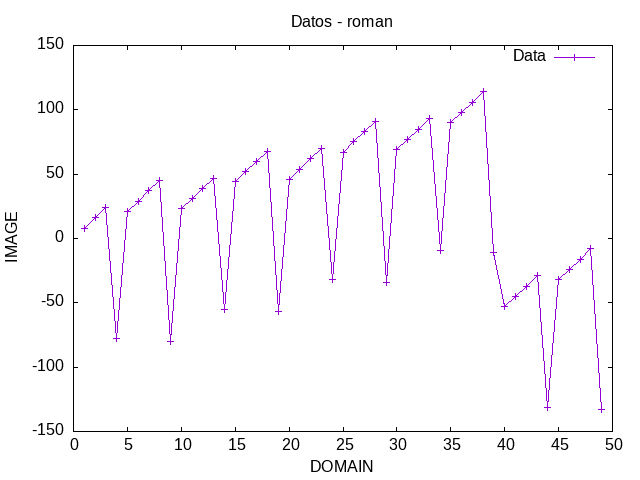
\includegraphics[width=0.3\linewidth]{img/roman/roman(49).png}}
    \subfloat[1 to 99]{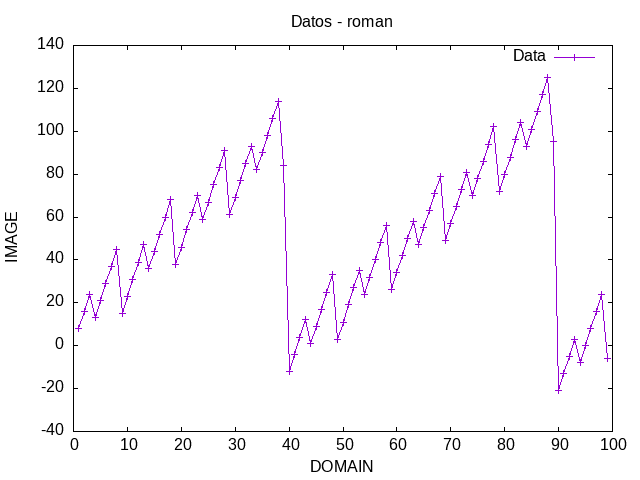
\includegraphics[width=0.3\linewidth]{img/roman/roman(99).png}}
    \subfloat[1 to 399]{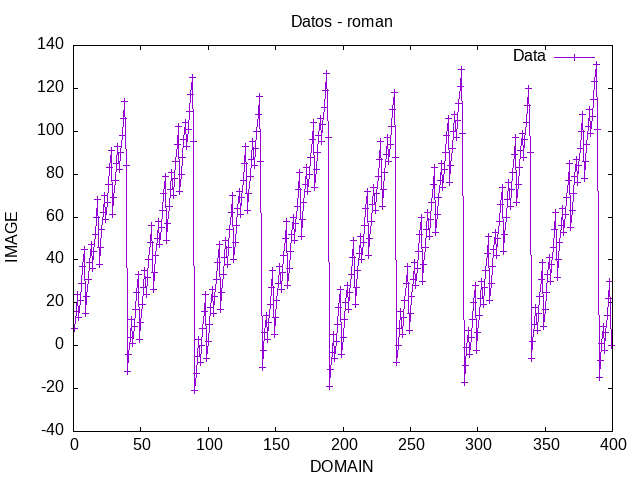
\includegraphics[width=0.3\linewidth]{img/roman/roman(399).png}}
    \caption{Distribution of the associated Arabic number to the Roman natural number}
    \label{romans}
\end{figure}\\
The function distribution that appears is the result of applying the function defined to the deterministic rules of Roman numbers, therefore there is no knowledge of which is the function behind this process.\\
However is an ideal case to use the experimental observation and try to obtain with the dataset given by the deterministic method a function that approximates the distribution of the dataset.

\subsection{Analisis of the dataset and creation of the neural network} 
The shape of the function shown in \ref{romans} tends to mimic the \textit{Sawtooth wave} but, in this case, it is not exactly periodical. This consequence (not being periodical) creates some problems because the application of the architecture developed to approximate the periodical functions can not be applied correctly.\\
Despite this problem, it is possible to use the architecture developed for periodical functions (tending to approach the \textit{Fourier Serie} of the \textit{Sawthooth wave}) in what seems to be the period of the wave $T=49$. \\
Therefore, the neural neural network should have the architecture shown in \ref{roman-architecture}.
\begin{figure}[h]
    \begin{minipage}{5.5cm}
        \begin{center}
            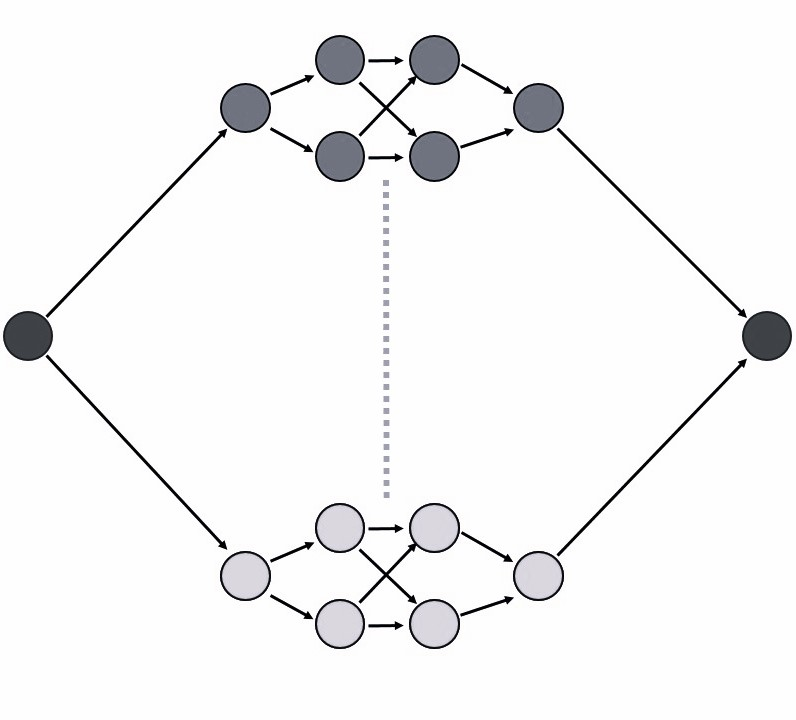
\includegraphics[width = 1\linewidth]{Neural_Network/roman_architecture.jpg}
            \caption{Working Hypotesis architecture of the neural network that approximates the Roman number distribution}
            \label{roman-architecture}
        \end{center}
    \end{minipage}
    \hspace{1em}
    \begin{minipage}{9cm}
 This neural network will be composed of two neurons (one input and one output) that send/receive the information to/from sub-neural networks with the architecture obtained to modulate the $\sin$ function.\\
 The neural network will be trained with only the first subset of the dataset (number between 0 and 49) and if a bigger number is introduced it only needs to be reduced as the remainder of the division of this number and the period $T$.\\
 The important part of the network is the number of sub-neural networks, the learning rate and the number of epochs that need to approximate properly the distribution.\\
 Unfortunately, the number of epochs and learning rate can not be deduced until it has been tested several times.
    \end{minipage}
\end{figure}\\
However, the number of sub-networks could be deduced as the amount needed to approximate the \textit{Fourier Serie} the \textit{Sawthooth wave} with enough precision.\\
To test and deduce the optimal number of sub-networks and the value of the learning rate, two similar approaches have been done, as can be seen in \ref{first-approach}
\begin{figure}[h]
    \centering
    \subfloat[Network with 3 architectures $1-2-2-1$ and fixed learning rate]{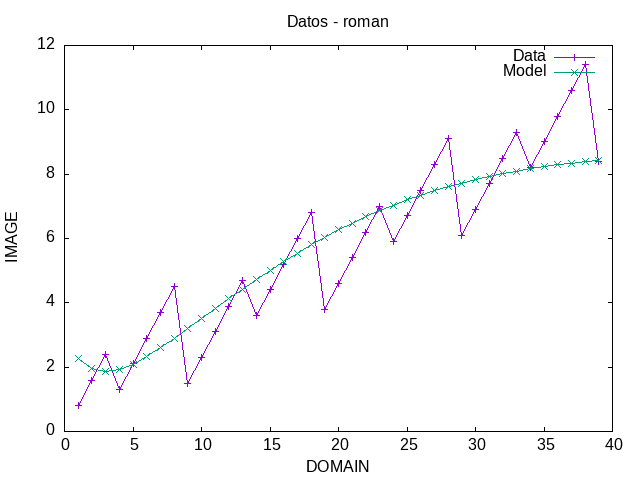
\includegraphics[width=0.45\linewidth]{img/roman/roman_first_approach.png}}
    \hspace{1em}
    \subfloat[Network with 4 architectures $1-2-2-1$ and decreasing learning rate]{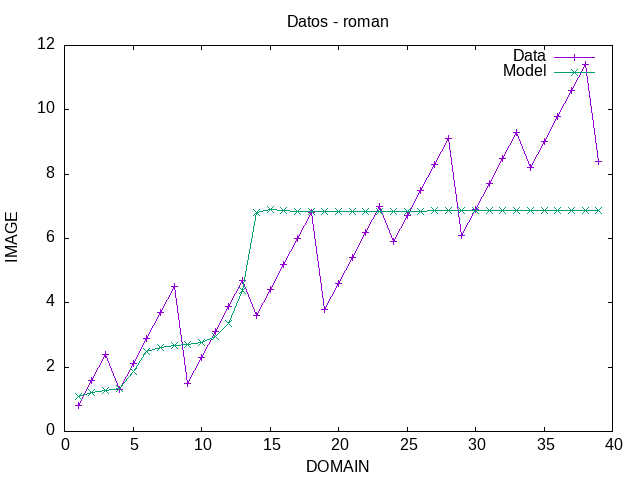
\includegraphics[width=0.45\linewidth]{img/roman/roman_second_approach.png}}
    \caption{Test of different neural networks to approach the distribution of Roman numbers}
    \label{first-approach}
\end{figure}\\
The conclusion obtained from this test is that the simple architecture of the $\sin$ function of $1-2-2-1$ is not enough and could be improved by using the most robust one of $1-2-4-1$.\\
Moreover, the variable learning rate (decreasing its value while the epochs increase) adjusts better the extrems of the distribution. However, the number of epochs tested (in the case of figure \ref{first-approach} $1000$) seem not to be enough.\\
Remark that the scale of the distribution has been decreased by one order of magnitude to reduce the variance between values and help to focus the Backpropagation when training (reducing the gradient vector to avoid erratic moves through the function cost).
\begin{figure}[h]
    \begin{minipage}{5.5cm}
        \begin{center}
            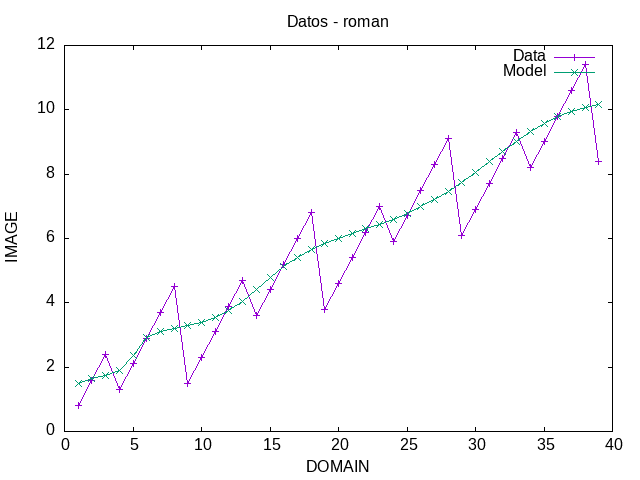
\includegraphics[width = 1 \linewidth]{img/roman/roman_third_approach.png}
            \caption{Improvement of sub-network capabilities to approach the roman numbers distribution}
            \label{second-approach}
        \end{center}
    \end{minipage} \hspace{1em}
    \begin{minipage}{9cm}
 If the test is repeated with 4 sub-networks with architectures $1-2-4-1$, introducing the learning rate reduction by one order of magnitude each time the number of epochs done increases its order of magnitude, and with $10000$ epochs the results obtained perform a better approach, as can be seen in \ref{second-approach}.\\
 From the figure, it is possible to deduce that the critical number of sub-networks has not been obtained yet. Moreover, observing the figure another conclusion can be made; the number of epochs is not enough.\\
 Nevertheless, it is possible that the model is more complex than it should be.
    \end{minipage}
\end{figure}\\
Studying the distribution and behaviour of the Roman numbers, it can be deduced that it has 3 subperiods.
The first period occurs when the number ends in $4$, the second when the number ends in $9$ and the third period is when the number starts with $4$ or $9$.
Using this information can be considered that the exact amount of subnetworks of the type $1-2-4-1$ to perform the best relation with precision-efficiency is $3$ (one for each period).
\begin{figure}[h]
    \begin{minipage}{5.5cm}
        \begin{center}
            \includegraphics[width = 1 \linewidth]{img/roman/roman_over_kill.png}
            \caption{Final architecture proposed to approach the distribution of roman numbers}
            \label{overkill-approach}
        \end{center}
    \end{minipage} \hspace{1em}
    \begin{minipage}{9cm}
        In this approach, the number of epochs has been increased to $10^6$ epochs and includes $3$ sub-networks with architectures $1-2-4-1$.
        The results obtained in \ref{overkill-approach} are not as good as was expected but give the best precision at the moment.
        However, until now there is not enough precision to consider any of these architectures a good candidate to approximate the distribution of the Roman numbers.
        Notwithstanding, all this unexpected non-approximation of the function could be caused by the unknown correct values of necessary epochs and/or learning rate.
    \end{minipage}
\end{figure}\\
This problem could not be solved using the Working Hypotesis and gives problems when planning the correct architecture for modelling a process.\\
Therefore, as it is impossible to perform a comparison between the results of the methods due to the poor precision of the models, an analysis of training cost has to be done to verify if it is practical to make improvements in the process to allow the models to train with more capabilities (such as parallelization using GPU, improvements of the neural network code or more data an training time). 

\newpage
\subsection{Efficiency and time-cost results}
To sum up, for all four tests we can reflect results\footnote{The results, studies and figures that have been shown/mentioned in the report where using a Raspberry PI 4 to ensure that the computational cost and time process can be completed without any problems of different capabilities.} in the table \ref{efficiency-table}, where the \textit{Training time} units is seconds.\\
\begin{table}[h]
    \centering
    \begin{tabular}{c|c|c|c|c|c}
 Sub-networks & Architecture & Epochs & Learning rate & Training time & Mean MSE\\\hline\hline
 3 & $1-2-2-1$ & $10^3$ & 0.01 & 1.03" & 4.09 \\\hline
 4 & $1-2-2-1$ & $10^3$ & $\{10^{-2}, 10^{-3}\}$ & 1.70 & 2.96 \\\hline
 4 & $1-2-4-1$ & $10^5$ & $\{10^{-(2+i)}\}_{i=0}^{2}$& 121.04 & 0.87 \\\hline
 3 & $1-2-4-1$ & $10^6$ & $\{10^{-(3+2i)}\}_{i=0}^{3}$& 617.55 & 0.14\\
    \end{tabular}
    \caption{Analysis of cost and efficiency about the different architectures develop}
    \label{efficiency-table}
\end{table}\\
It can be observed that the training models used are quite good taking into account that the epochs are "relatively low". Also, mention that the "size" of the architecture is not as big as normally MLPs are done to approach this type of problem.\\
Therefore it can be considered a shred of evidence that the Working Hypothesis made as a set of "considerations" to develop neural networks could be verified in other dimensions and consolidated as a theorem if it is possible to prove its properties.\\
In the worst scenario, the study has shown that knowing the process behind a model can be used as a sustain to create neural network experts in solving this process (which could perform a fixed amount of operations to develop a task which, in its deterministic process of calculation, will not be able to determine or even have the solution in a reasonable amount of time).

\newpage
\section{Conclusions}
All the objectives initially planned have been achieved:
\begin{enumerate}
    \item Develop neural networks using C language coding.
    \item Propose a possible improvement of how neural networks can be designed.
    \item Verify that The \textbf{Universal Approximation Theorem} definition can be expanded and used in cases that theoretically it should not be able to.
    \item Propose a neural network using the obtained Working Hypotesis that approximates a deterministic process.
\end{enumerate} 
In spite of the fact that the most challenging objective, being able to improve the time process for a deterministic process using a neural network, was not achieved,
during the study, it has been shown that there exists enough evidence that this challenge can be done with a better performance and analysis of the deterministic processes.\\
It is unfair not to mention that the deterministic process selected to verify the improvements of applying neural networks was not as easy as it was thought and with another deterministic process this verification objective could have been achieved much easily.\\
Also, emphasize that the different Working Hypoteses done during the study can be an initial point for future studies.\\
Encouraging everyone to take it as a starting point to develop better the Working and Suggested Hypothesis and correct any possible mistakes that could have been done and not taken into consideration.\\

\newpage
\begin{thebibliography}{X}
\bibitem{WIKIPEDIA-MLP} \textsc{Wikipedia},
\textit{Multilayer perceptron},\\ \url{https://en.wikipedia.org/wiki/Multilayer_perceptron}
\bibitem{WIKIPEDIA-PERCERPTRON} \textsc{Wikipedia},
\textit{Perceptrón},\\ \url{https://es.wikipedia.org/wiki/Perceptr%C3%B3n}
\bibitem{WIKIPEDIA-ACTIV.FUNCT,} \textsc{Wikipedia},
\textit{Activation function},\\ \url{https://en.wikipedia.org/wiki/Activation_function}
\bibitem{WIKIPEDIA-FRANK} \textsc{Wikipedia},
\textit{Frank Rosenblatt},\\ \url{https://es.wikipedia.org/wiki/Frank_Rosenblatt}
\bibitem{WIKIPEDIA-ACTIVATINGFUNCTION} \textsc{Wikipedia},
\textit{Activating Function},\\ \url{https://en.wikipedia.org/wiki/Activating_function}
\bibitem{WIKIPEDIA-ART.NN} \textsc{Wikipedia},
\textit{Artificial neural network},\\ \url{https://en.wikipedia.org/wiki/Artificial_neural_network}
\bibitem{WIKIPEDIA-NN} \textsc{Wikipedia},
\textit{Neural network},\\ \url{https://en.wikipedia.org/wiki/Neural_network}
\bibitem{WIKIPEDIA-SIGMOID_TEOREM} \textsc{Wikipedia},
\textit{Universal Approximation Theorem},\\ \url{https://en.wikipedia.org/wiki/Universal_approximation_theorem}
\bibitem{WIKIPEDIA-MSE} \textsc{Wikipedia},
\textit{Mean Squared Error},\\ \url{https://en.wikipedia.org/wiki/Mean_squared_error}
\bibitem{WIKIPEDIA-MAE} \textsc{Wikipedia},
\textit{Mean Absolute Error},\\ \url{https://en.wikipedia.org/wiki/Mean_absolute_error}
\bibitem{WIKIPEDIA-CE} \textsc{Wikipedia},
\textit{Cross-Entropy},\\ \url{https://en.wikipedia.org/wiki/Cross-entropy}
\bibitem{WIKIPEDIA-BACKPROP} \textsc{Wikipedia},
\textit{BackPropagation},\\ \url{https://en.wikipedia.org/wiki/Backpropagation}

\bibitem{Dan} \textsc{Dantzig, G.B.} y \textsc{P. Wolfe},
<<Decomposition principle for linear programs>>,
\textit{Operations Research}, \textbf{8}, págs. 101--111, 1960.

\end{thebibliography}
\end{document}
